%入口页

\documentclass[master]{thesis-uestc}
%
  \usepackage{booktabs}% 三线表
  \usepackage{tabularx}% 让表格自适应宽度与自动换行
  \newcolumntype{Y}{>{\centering\arraybackslash}X}% 定义自适应列的居中格式 Y, 用 X 为左对齐(自适应列)
  \usepackage{xcolor}% 颜色宏包
  \usepackage{listings}% 代码高亮
  \definecolor{codegreen}{rgb}{0,0.6,0}
  \definecolor{codegray}{rgb}{0.5,0.5,0.5}
  \definecolor{codepurple}{rgb}{0.58,0,0.82}
  \definecolor{backcolour}{rgb}{0.95,0.95,0.92}
  \lstset{
      commentstyle=\color{codegreen},
      keywordstyle=\color{magenta},
      stringstyle=\color{codepurple},
      basicstyle=\footnotesize,% 代码字体大小
      breakatwhitespace=false,% 是否只在空白字符处断行
      breaklines=true,% 自动断行
      captionpos=b,% 标题位置为 bottom
      keepspaces=true,
      numbers=left,% 行号的位置
      numbersep=5pt,% 行号与代码的距离
      numberstyle=\tiny\color{codegray},% 行号样式
      stepnumber=2,% 隔行显示行号
      showspaces=false,
      showstringspaces=false,
      showtabs=false,
      tabsize=2
  }
  \newcommand\keyword[1]{\colorbox[rgb]{0.9,0.9,0.9}{#1}}
  % \usepackage{underscore}% 处理下划线问题

  \title{基于微擎的微信商城 H5 开发}
  \author{宋云超}

\begin{document}

  % 中文摘要

\begin{chineseabstract}
  如今,互联网+ 的新型商业模式正在迅速发展,微信平台又给 App 的开发提供了新的模式——微信商城模式。
  \par
  本项目开发了一款移动端的 App Demo, 采用了最新的 H5 技术,充分利用了微信公众号平台的优势,让用户通过关注公众号即可进入商城而不需下载。此款应用实现了三大基本功能:商城功能、文章推送、信息记录,客户在商城模块可以浏览商品、进入店铺、完成下单与支付操作;在文章模块可以浏览文章、查看文章、点赞和收藏文章;在信息记录模块可以查看自己的消费记录、收藏记录以及信息设置等。
  \chinesekeyword{商城,前端,微信}
\end{chineseabstract}

%    -- 中文摘要
  % 英文摘要

\begin{englishabstract}% 英文摘要
  Nowadays, a whole-new bussiness model named "Internet Plus" is developing rapidly, and wechat app, with great potential, is providing a perfect paltform for app development called wechat store.
  \par
  This project has developed an app demo, using advanced h5 technique, based on wechat public account. Customers can access this app via public account. This app has implemented three fundamental functions——online shopping, articles posting and record maintaining. Customers can look through the store list, choose services they want, order and pay in the online shopping module. In article module, Customers can look through the article list, read artiles, like and collect them. Consuming records, collection and settings are kept in the record module.\\
  \englishkeyword{store, wechat, public, account}
\end{englishabstract}
%    -- 英文摘要
  \thesistableofcontents% -- 目录

  % chapter: 绪论

\chapter{绪论}
  \label{chap:绪论}
    \section{课题背景与现状}
      \label{sec:课题背景与现状}
        \subsection{互联网+}
          \label{subsec:互联网_}
            2015 年 3 月 5 日,李克强总理在十二届人大三次会议上提出了“互联网+”的概念。“互联网+”的实质就是:互联网+传统行业。越来越多的企业与互联网结合,开辟了全新的经营模式————线上线下模式,线上接单,线下服务。如今这种商业模式已经深入到我们生活的方方面面,大量的企业开发了自己的商城网站,也开发了移动端的 App, 让我们的生活更加便捷,出行有滴滴,携程,购物有淘宝天猫,娱乐有美团等,这些应用让我们可以不受时间和空间的约束,去享受企业的便利服务。

        \subsection{微信平台}
          \label{subsec:微信平台}
            微信平台的出现为企业发展带来了新的机遇。微信平台有着超过 4 亿的用户基础,如此大的用户量蕴藏着巨大的价值。微信的价值主要在以下两点:
            \begin{itemize}
              \item 传播迅速
              \item 平台接口
            \end{itemize}
            \par
            传播迅速。我们知道,一副世界地图只需要 4 中颜色就可以表示出世界上几百个的国家,而不会产生混淆,这就是著名的四色理论。同样,在人脉的研究中也有个著名的理论——六度人脉理论,即一个人和世界上任何一个陌生人之间最多不超过 6 个陌生人,因此,如果一个企业把产品与服务做好,在自己的朋友圈取得信任后,就可以在圈内迅速传播,短时间内就可以打造企业的知名度。
            \par
            平台接口。传统的 App 必须要让客户去下载安装,而微信平台提供的网页接口可以让用户无需下载 App,用户关注公众号后就可以通过链接或菜单进入商城,直接下单购买,甚至省去了注册的步骤,因为微信平台可以获取用户的信息从而自动完成注册。

        \subsection{医疗大数据}
          \label{subsec:医疗大数据}
            而最近几年,健康医疗行业也迅速发展起来,2014 年,马云又投资10亿,拿下全国400家医院,覆盖90\% 的省份,我们可以看到其对健康医疗行业的重视。人们也在更多的关注健康与保健。而随着互联网的兴起的大数据行业也在迅速发展。海量的数据蕴含着丰富的信息,依据数据理论,通过一定的算法,就可以从数据中挖掘有价值信息。
            对健康状况的预测是大数据与医疗行业的一个重要的结合点。通过的先进的医疗器械获取大量患者的身体的各项指标,然后基于以往海量的样本进行数据建模,利用分类算法,就可以对一个人的健康状况作出比较精准的评估,进而对患者进行健康指导。

    \section{理论与技术}
      \label{sec:理论与技术}
        最近移动应用炒的最火的就是 H5 技术。H5 从狭义上说就是 HTML5,即最新版的 HTML 技术,从广义上说则是包含了 HTML5, CSS3, ES5甚至ES6在内的前端技术及框架,这些技术和框架可以让开发者迅速开发出华丽的移动应用。
        \par
        H5 相对于 H4 增加了很多新的特性,例如更多语义标签、canvas 绘图、多媒体标签、更强大的本地存储等;CSS 3 相对于上个版本功能更加多样化,弹性盒子模型、CSS 动画等;ES 指的是 JavaScript 的标准版本,最新的 ES6 相对于 ES 5 也有了更多扩展,如块作用域、of 语法、generator 函数等,不过还未大量采用,但一些最新的框架已经采用 ES6 开发了。这些只是底层的技术,要实现复杂的应用需要稳定成熟的框架,框架的出现于发展让应用的开发更为便捷与迅速。

    \section{项目特色与意义}
      \label{sec:项目特色与意义}
        我们的商城采用最新的 H5 技术,旨在打造一个特色的商城:定制的页面,专一的产品,服务与产品结合等,通过公众号运营,而不是独立的 App。
        此应用可以同时为客户提供服务与产品的信息,主要有两大门店:专注服务的门店与专注产品的门店,服务主要是基于艾灸的保健服务,产品主要是基于艾草的各种产品,如:艾绒棒、艾草保健品等,当然后期的服务与产品中还会继续扩展。应用同时设有艾灸百科专栏,让用户更多的了解艾灸文化,最后,应用还会专门记录客户的保健记录,重点不在于消费记录,而是健康状况记录,根据客户每次保健采集的指标,通过后台的大数据分析,评估健康状况,不过这些是以后的扩展功能。
        \par
        此项目的开发对我来说是一次难得的锻炼机会,让我在技术上有了很大提升。而且,此项目与我的职业道路紧密相关,我选择的职业就是前端开发,通过做项目,让我在公司入职之前给自己提前做了培训,为公司的入职做好准备。

    \section{发展趋势}
      \label{sec:发展趋势}
        个人认为,移动应用的发展有如下的趋势:
        \begin{itemize}
          \item 更多采用公众平台甚至小程序
          \item 专一化与定制化
        \end{itemize}
        \par
        上面提到,目前的移动开发越来越倾向于在微信平台开发,利用微信平台提供的巨大优势,可以让企业更快地推广、传播。现在有一种理论认为,企业的发展越来越向工匠化发展,即企业的价值更多地在于把产品做精,在精而不在多,这样产品就有了更多的品牌价值与权威性,做就做到最好,同时,为此开发的移动应用的就会越来越针对某种产品专门开发,这样的应用非常专一,而且轻量级。这样的应用还有一个特色,就是更强的定制性,有自己的创意,权威与特色这两大要素结合,让企业在未来竞争中更容易生存。



%        -- 绪论
  % % Chapter: 需求分析

\chapter{需求分析}
  \label{chap:需求分析}

\section{综述}
  \label{sec:综述}
    我的项目是开发一个商城,分为三大模块,分别由三个底部菜单进入。第一大模块是商城部分,由一个列表展现页、店铺详情页、支付详情页和支付成功页组成,可以实现完整的一套购买流程:进入商城 -> 填写订单 -> 支付 -> 支付成功。第二大模块是艾灸文化部分,主要用来推送软文,传播艾灸保健的文化,扩展人们的知识面,由一个文章列表页和文章详情页组成,文章详情页中可以给文章点赞、收藏等。第三大模块则是我的空间部分,保存了个人的基本信息、收藏与保健记录等。
    \par
    每个页面都有自己的设计图,这是由设计师设计的,我主要负责用代码一行一行去实现各个样式细节,并且还要有交互功能以及各个页面的业务逻辑,下面就来一一介绍各个要页面的功能。

\clearpage
\section{商城模块}
  \label{sec:商城模块}
    \subsection{首页}
      \label{subsec:首页}
        我们先来看下首页的设计图(\ref{fig:home_dsn}),首页是客户打开商城时默认进入的页面,从服务器获取数据信息,以列表的形式展现商城的一些基本信息,包括店铺的缩略图、店名、艾灸服务的价格、其他一些服务及价格、店的地理位置等,而且可以判断根据按钮的颜色判断客户是否在商城预定过,然后点击商城就可以进入店铺内部。
        \begin{figure}[htbp]
          \centering
          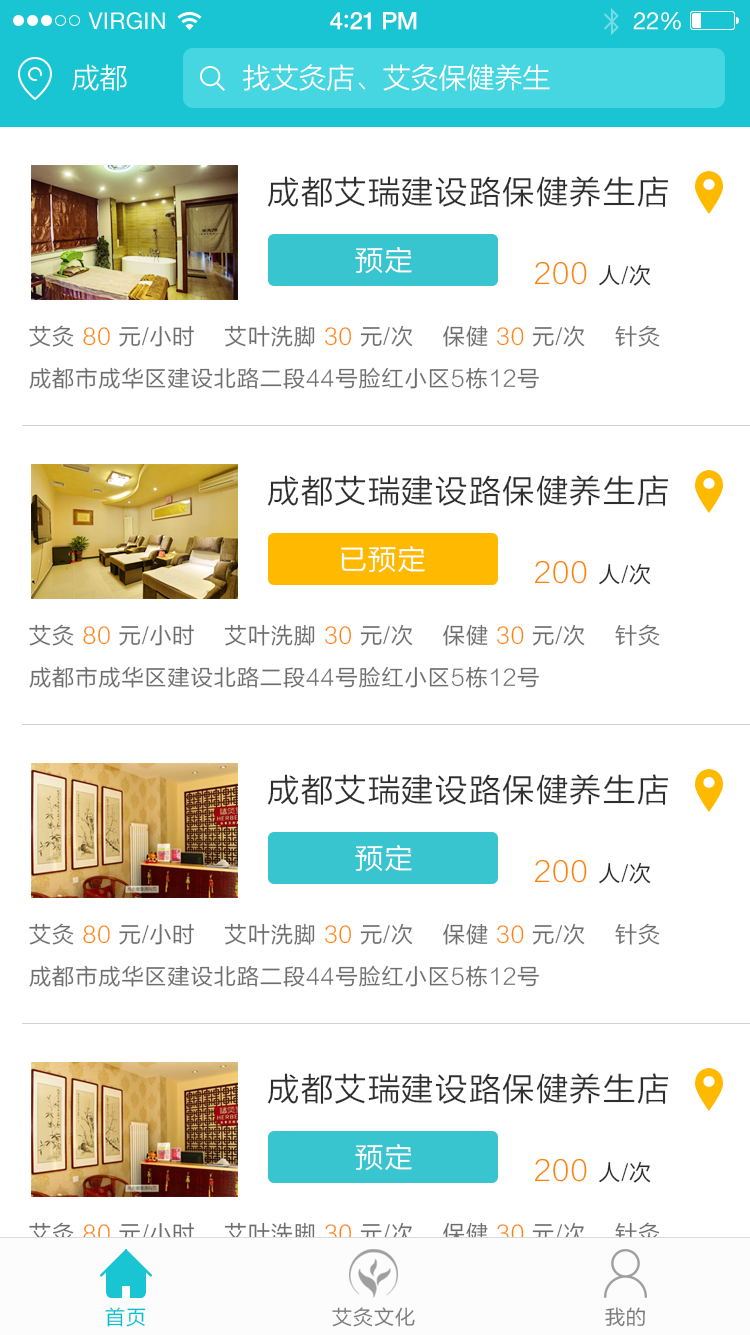
\includegraphics[width=8cm]{./img/home_dsn.jpg}
          \caption{首页的设计图}
          \label{fig:home_dsn}
        \end{figure}

    \subsection{店铺详情页}
      \label{subsec:店铺详情页}
        店铺详情页与下一页的支付页是一个完整的下单与支付流程。店铺详情页展示了一个店铺内部的详细信息,如图(\ref{fig:strdetail_dsn}),包括店铺的内部装饰图、店铺的具体的服务与价格,客户可以在这里勾选服务与预定的日期,以及进行预定操作,预定过程下一页还会继续,用于填写个人的基本信息。
        \begin{figure}[htbp]
          \centering
          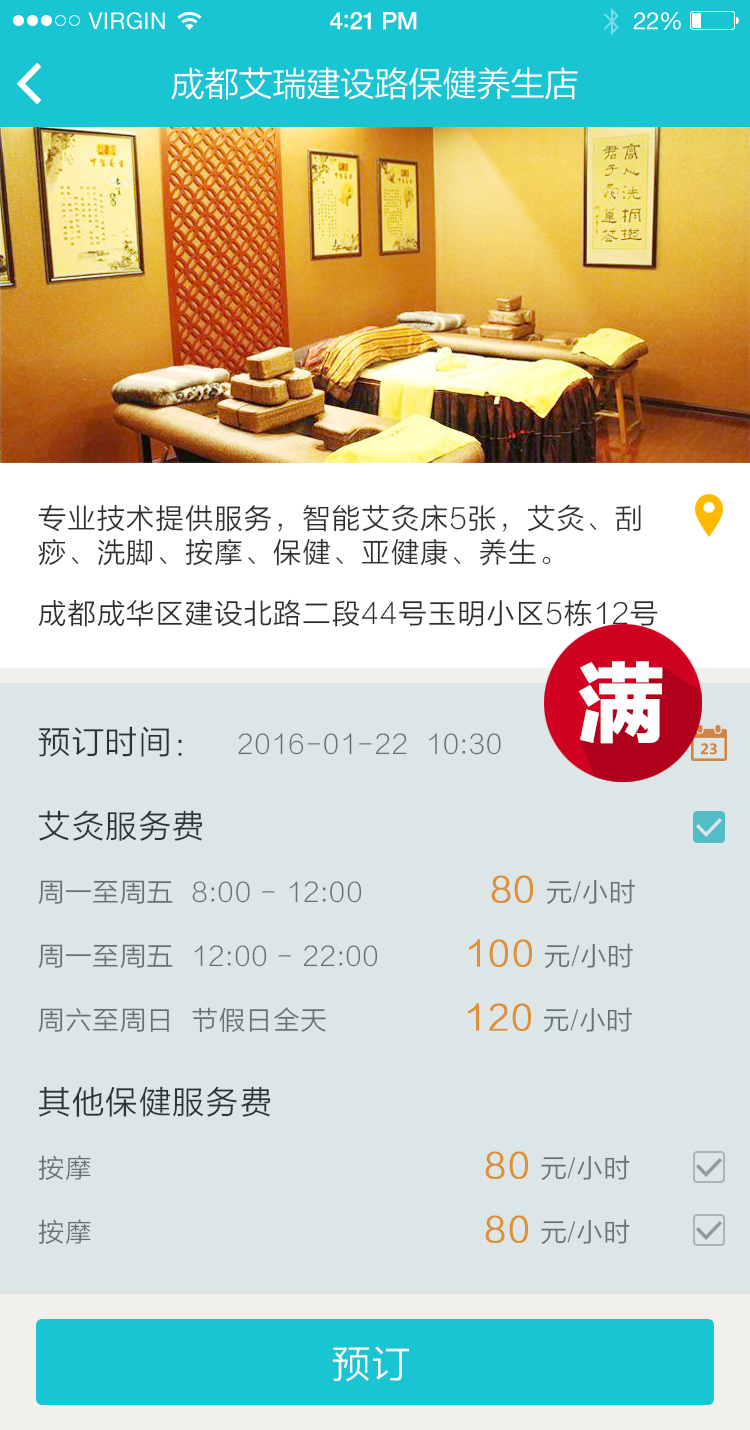
\includegraphics[width=8cm]{./img/strdetail_dsn.png}
          \caption{店铺详情页的设计图}
          \label{fig:strdetail_dsn}
        \end{figure}

    \subsection{支付页}
      \label{subsec:支付页}
        支付页继续上一页的操作,支付页的设计图如图(\ref{fig:pay_dsn}),上一页主要选择了预定的服务,这一页来选择各个服务的人数,选择人数的同时,上面的总价一栏会实时显示总价;接下来是个人信息的填写,包括姓名与电话;最后是选择支付方式,支持微信和支付宝支付,点击最后的支付按钮即可完成支付,并跳转到支付成功的提示页面。
        \begin{figure}[htbp]
          \centering
          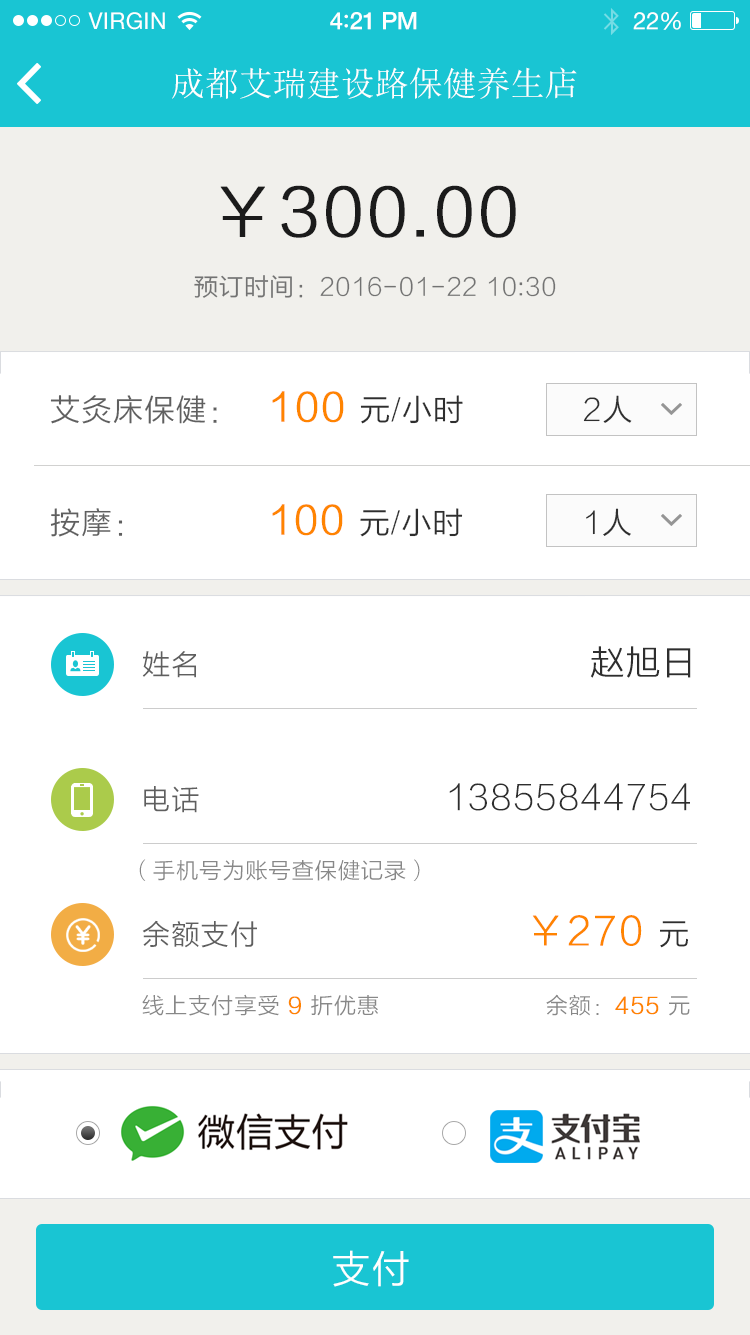
\includegraphics[width=8cm]{./img/pay_dsn.png}
          \caption{支付页设计图}
          \label{fig:pay_dsn}
        \end{figure}

    \subsection{支付成功页}
      \label{subsec:支付成功页}
        支付成功页主要功能除了提示客户已经购买成功,还包括了分享功能,如图(\ref{fig:pay_successful_dsn}),可以分享到微信、微博、QQ 空间,分享成功的同时可以奖励艾灸币,提交到服务器保存,客户可以用来兑换现金。
        \begin{figure}[htbp]
          \centering
          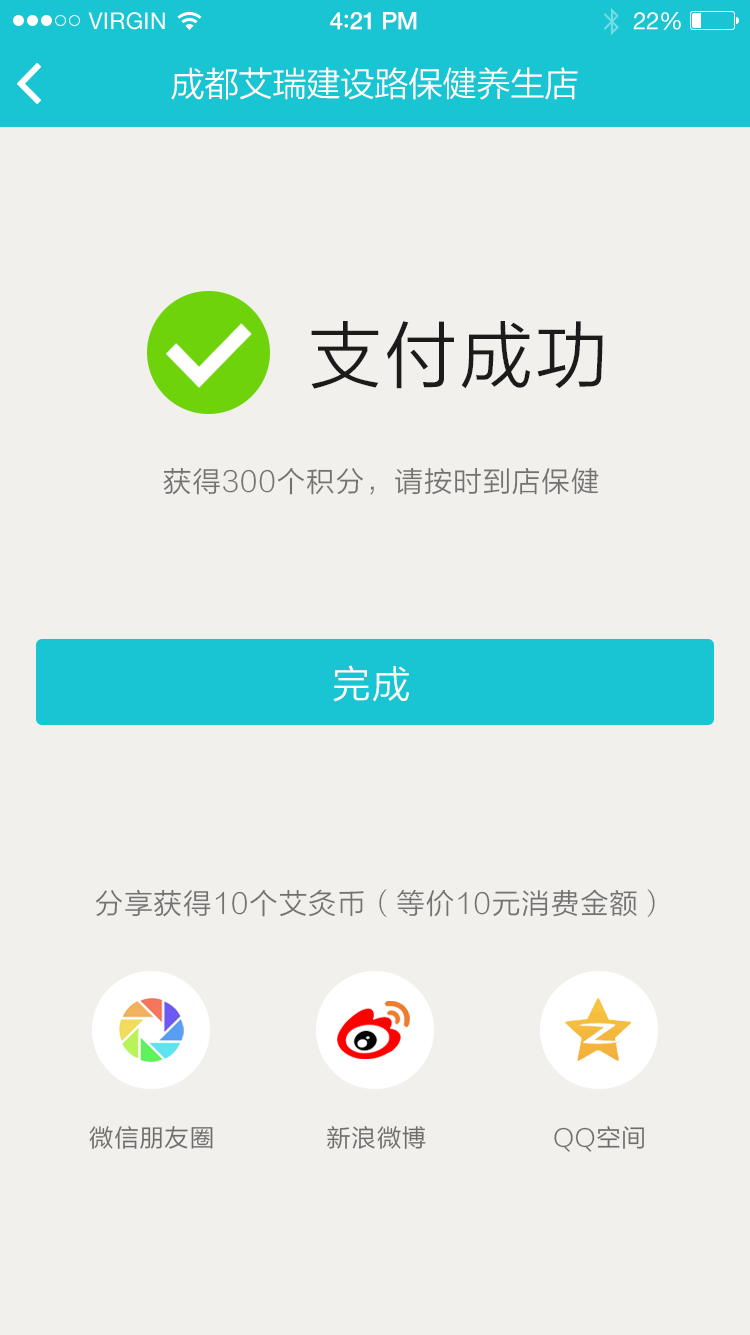
\includegraphics[width=8cm]{./img/pay_successful_dsn.png}
          \caption{支付成功页的设计图}
          \label{fig:pay_successful_dsn}
        \end{figure}

\clearpage
\section{文章模块}
  \label{sec:文章模块}
    \subsection{文章列表页}
      \label{subsec:文章列表页}
        文章列表页的设计图如图(\ref{fig:artlist_dsn}),
        \begin{figure}[htbp]
          \centering
          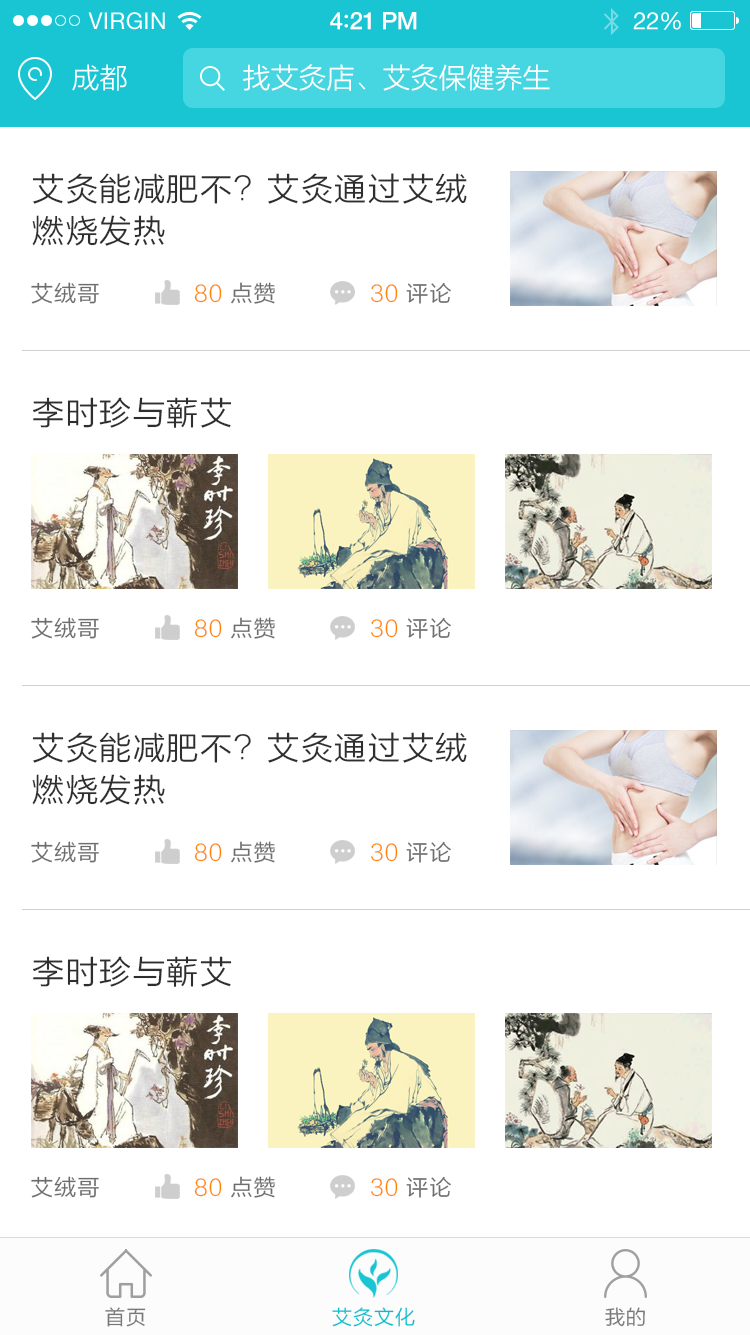
\includegraphics[width=8cm]{./img/artlist_dsn.png}
          \caption{文章列表页的设计图}
          \label{fig:artlist_dsn}
        \end{figure}
        此页面以列表的形式展示了最近的一些文章,每项都显示了文章的一些简要信息,如文章标题、图片、作者、点赞数与评论数等,点击就可进入文章的详情页。


    \subsection{文章详情页}
      \label{subsec:文章详情页}
        文章详情页的设计图如图(\ref{fig:artdetail_dsn}),客户可以在此页浏览文章,喜欢的话可以点击上面的点赞收藏图标进行收藏,收藏的文章会保存在我的空间的收藏一栏的位置。
        \begin{figure}[htbp]
          \centering
          
\includegraphics[width=8cm]{./img/artdetail_dsn.png}
          \caption{文章详情页的设计图}
          \label{fig:artdetail_dsn}
        \end{figure}

\clearpage
\section{我的空间模块}
  \label{sec:我的空间模块}
    \subsection{我的空间页}
      \label{subsec:我的空间页}
        我的空间页的设计图如图(\ref{fig:mine_dsn}),此页展示了用户的一些基本信息,如昵称、头像,还通过气泡提示的方法展示了客户保健的次数、收藏的店铺和文章的个数以及积分数。下半部分是一些导航菜单,分别可以进入个人的消费记录页面、我的收藏页面、设置信息的页面。
        \begin{figure}[htbp]
          \centering
          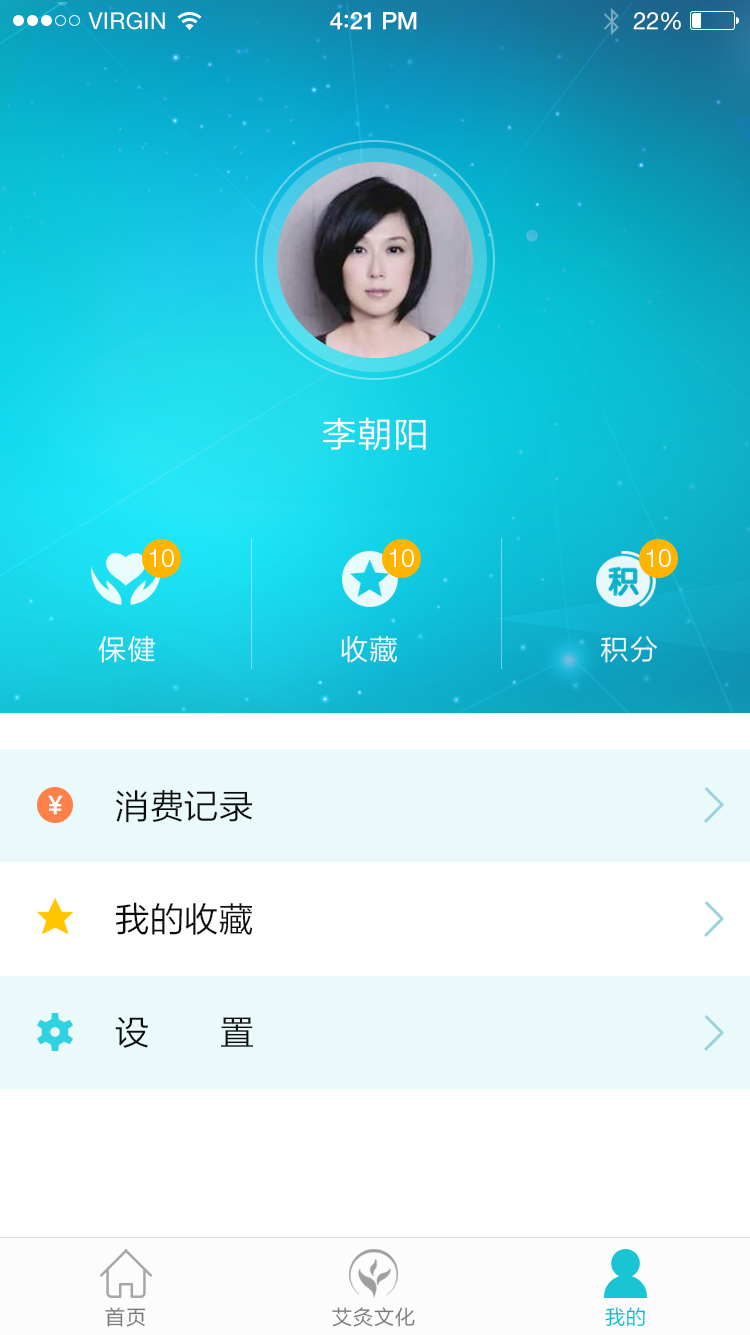
\includegraphics[width=8cm]{./img/mine_dsn.png}
          \caption{我的空间页}
          \label{fig:mine_dsn}
        \end{figure}

    \subsection{消费记录页}
      \label{subsec:消费记录页}
        消费记录记录了个人的消费情况,以流水线的样式展现,展示的信息包括店名、保健的人数、时间、费用以及积分等,积分将来可以用于兑换艾灸币,顶部还展示了总的消费情况,总的积分。设计图如图(\ref{fig:record_dsn})。
        \begin{figure}[htbp]
          \centering
          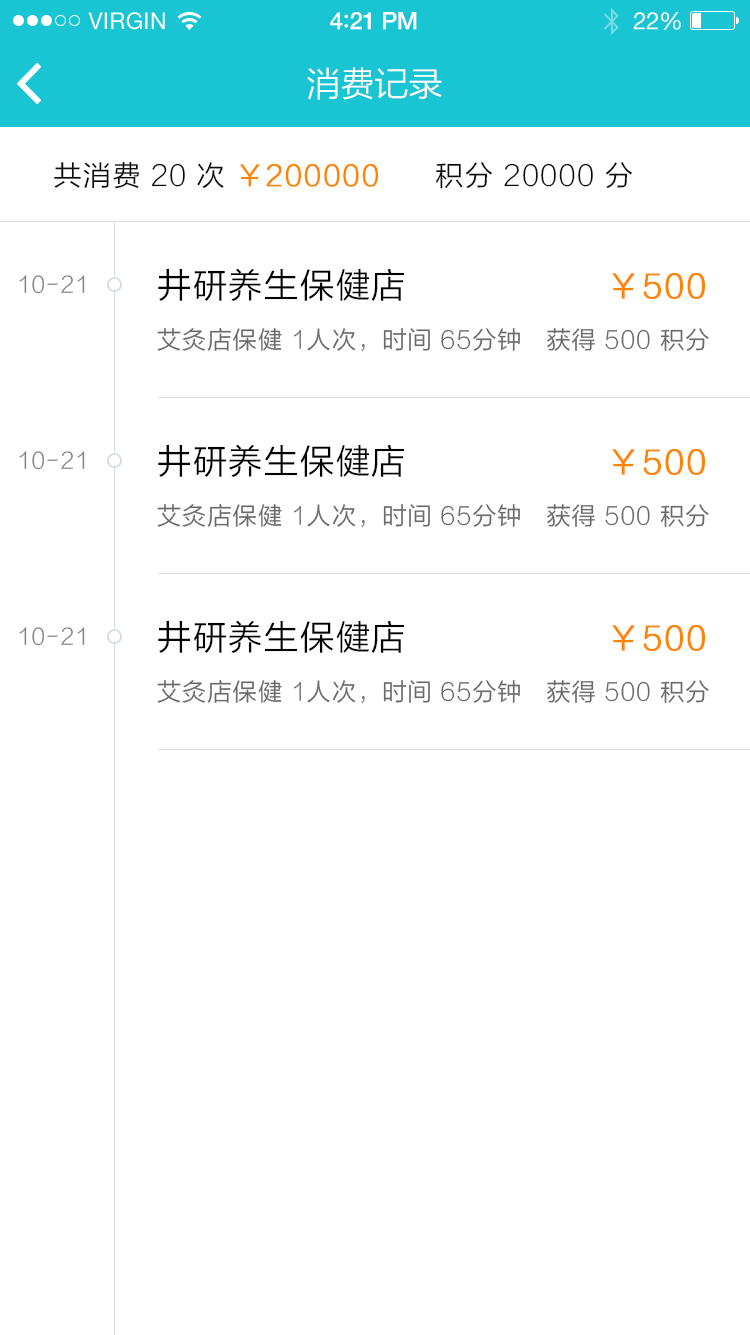
\includegraphics[width=8cm]{./img/record_dsn.png}
          \caption{消费记录页}
          \label{fig:record_dsn}
        \end{figure}

    \subsection{设置页}
      \label{subsec:设置页}
        设置页的设计图如图(\ref{fig:setting_dsn})在这一页中,客户可以设置自己的基本信息,包括昵称、手机号、登录密码等。
        \begin{figure}[htbp]
          \centering
          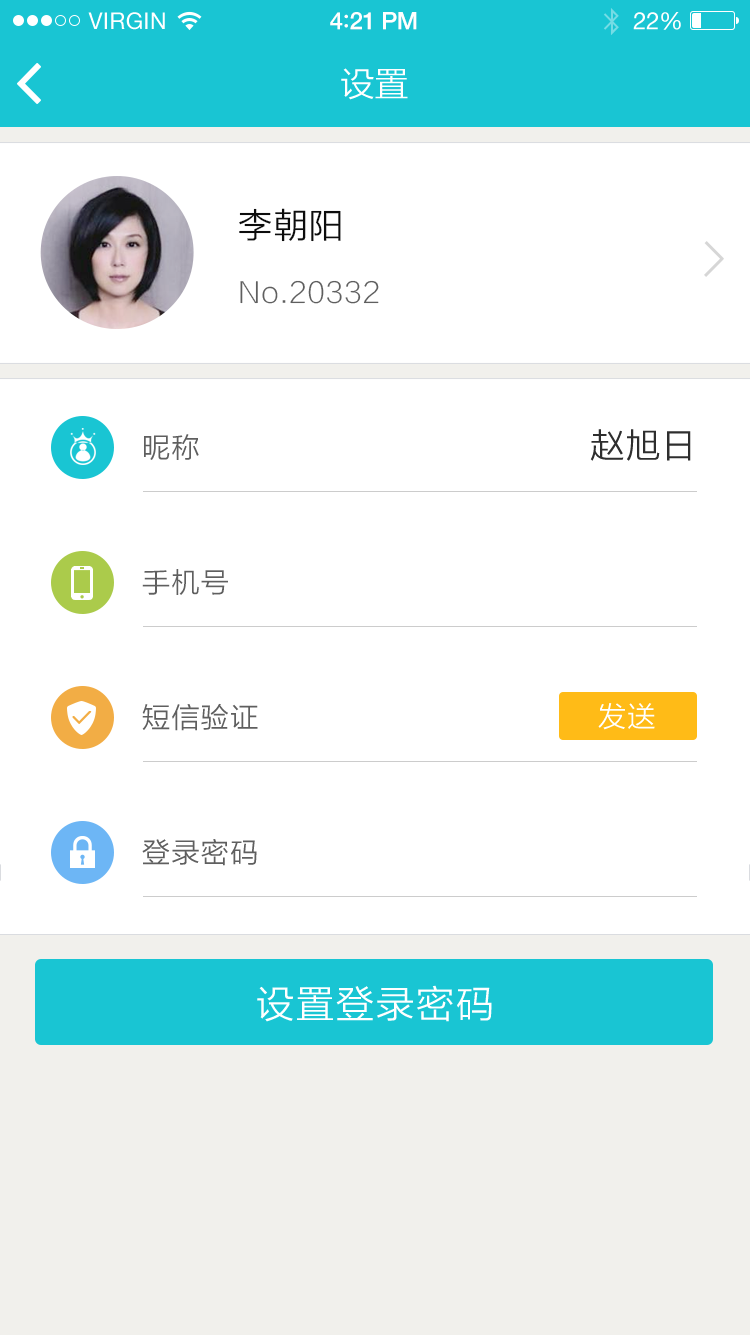
\includegraphics[width=8cm]{./img/setting_dsn.png}
          \caption{设置页的设计图}
          \label{fig:setting_dsn}
        \end{figure}

\clearpage
\section{本章小结}
  \label{sec:需求小结}
    本章结合设计图分析了项目的基本需求,展示了一个网上商城应该具备的基本功能。有了基本需求就可以开发了,不过开发前需要进行充足的准备,包括基本知识技能的学习、工具的选择与使用,下面一章我们就来简要介绍项目开发用到的必要知识与工具。

%    -- 需求分析
  % % 项目用到的技术与工具简介

\documentclass[UTF8]{ctexbook}
%
  \ctexset{
      part/number = \chinese{part}% 用于解决 part 的标号不显示问题
  }
  \usepackage{hyperref}% 超链接
  \hypersetup{
      colorlinks=false,% 去掉超链接颜色
      pdfborder=0 0 0% 取消超链接的边框
  }
  \usepackage{graphicx}% 图片管理
  \graphicspath{{images/}}% 设置图片搜索路径
  \usepackage{float,varwidth}% 浮动体
  \usepackage{booktabs}% 三线表
  \usepackage{tabularx}% 让表格自适应宽度与自动换行
  \newcolumntype{Y}{>{\centering\arraybackslash}X}% 定义自适应列的居中格式 Y, 用 X 为左对齐(自适应列)
  \usepackage{fancyhdr}% 页眉设置
  \usepackage{xcolor}% 颜色宏包
  \usepackage{listings}% 代码高亮
  \definecolor{codegreen}{rgb}{0,0.6,0}
  \definecolor{codegray}{rgb}{0.5,0.5,0.5}
  \definecolor{codepurple}{rgb}{0.58,0,0.82}
  \definecolor{backcolour}{rgb}{0.95,0.95,0.92}
  \lstset{
      commentstyle=\color{codegreen},
      keywordstyle=\color{magenta},
      stringstyle=\color{codepurple},
      basicstyle=\footnotesize,% 代码字体大小
      breakatwhitespace=false,% 是否只在空白字符处断行
      breaklines=true,% 自动断行
      captionpos=b,% 标题位置为 bottom
      keepspaces=true,
      numbers=left,% 行号的位置
      numbersep=5pt,% 行号与代码的距离
      numberstyle=\tiny\color{codegray},% 行号样式
      stepnumber=2,% 隔行显示行号
      showspaces=false,
      showstringspaces=false,
      showtabs=false,
      tabsize=2
  }
\begin{document}
  \chapter{技术、框架与工具}
    \label{chap:技术与工具}
      本章主要介绍了项目所用到的技术和工具,技术包括:
      \begin{itemize}
        \item HTTP
        \item JSON 与 XML
        % \item Apache 服务器的配置
        % \item Nodejs 与 npm
        % \item MongoDB
        \item 前端技术
        \item H5
        \item CSS3 与 Less
        \item ES5,ES6
        \item 前端库与框架
        \item jQuery
        \item Bootstrap
        \item MVC 与 AngularJS
      \end{itemize}

      工具包括:

      \begin{itemize}
        \item Sublime Text3
        \item Chrome
        \item 微信 Web 开发者工具
        \item Git
      \end{itemize}

    \section{技术与框架}
      \label{sec:技术框架}

        \subsection{HTTP}
          \label{subsec:http}
            \subsubsection{HTTP 简介}
              \label{subsubsec:http_简介}
                HTTP(HyperText Transport Protocol)是超文本传输协议,规定了浏览器和服务器的通信的规则。RFC 系列文档收录了互联网通信的一些规范,其中 RFC2612 记录了 HTTP 协议的规范。

                当我们在浏览器中键入了一个网址的时候,都发生了什么?首先浏览器把网址发送到某个 DNS 服务器,DNS 服务器负责将网址解析成 ip 地址,然后浏览器再向 ip 地址对应的服务器发送请求,服务器接收到请求,返回你想要的资源,通常是网页的形式。其实从服务器那边传过来的,不只有网页,还有一些头信息,这些信息对客户是不可见的,但却十分重要,这些信息反映了用到的 http 协议及其版本、缓存相关的设置、传输的编码等、获取信息的状态及状态码等,这些信息都可以从 Chrome 的调试工具里面看到。

            \subsubsection{开发者如何使用 HTTP}
              \label{subsubsec:开发者如何使用_http}
                理解 HTTP 协议对于网站开发者,无论是前端还是后台都十分重要。
                \par
                对于前端工作者,我们时常需处理与后台的数据传输问题,而与后台的交互离不开 Ajax (Asynchronous JavaScript And XML),我们开发用到的一些框架(如 jQuery)都集成了 Ajax 请求的方法,如果我们理解了 HTTP 协议,就不会对 Ajax 请求所需要的那些参数感到陌生,我们也常常遇到请求失败等的问题,此时我们就需要在浏览器中去查看 Get 请求或 POST 的构建是否正确。
                \par
                对于后台开发者,理解 HTTP 请求就更重要了,因为后台要负责 GET 请求和 POST 请求的接收和处理,需要设置 cookie 、回话管理、资源的缓存、缓存的时间等等。
                \par
                因此,我们如果要想开发网站,就要花时间去理解 HTTP 协议,这样才能让我们走得更远。

        \subsection{JSON 和 XML}
          \label{subsec:json_和_xml}
            \subsubsection{前后分离的开发模式}
              \label{subsubsec:前后分离的开发模式}
                现在的项目开发流行一种新模式,即前后端分离,这种开发方法可以降低耦合,提高开发效率,让不同的程序员更加专注自己擅长的地方,如后端工程师只需专注于数据的增删改查等数据库操作,前端只负责页面样式、动画特效等。前后端的数据采用的数据格式主要有两种:JSON 和 XML,主流都是在用 JSON,少部分仍在使用 XML,例如微信的开发。
            \subsubsection{XML}
              \label{subsubsec:XML}
                XML(Extensible Markup Language) 是表示数据的一种格式,特点是采用了类似 HTML 标签的方式把数据包裹起来,不同的地方在于标签名可以自定义,这有点类似 AngularJS 的自定义命令,XML 可以表示出所有的数据结构:对象和数组,语法严格,但是用 XML 标签构造的数据携带了大量的无用的标签,是 JSON 未出来之前的很流行的一种数据传输格式。尽管 JSON 更简洁,但 XML 还未完全退出,这里之所以提到 XML 是因为微信开发仍在采用,微信的事件推送、消息机制的 POST 数据,都是 XML 格式。
            \subsubsection{JSON}
              \label{subsubsec:JSON}
                JSON(JavaScript Object Notation, JavaScript 对象表示法) 是 JavaScript 语言的对象的表示方法,由 Douglas Crockford 提出的,《JavaScript: The Good Parts》的作者。JSON 数据格式十分简洁,只需 "{", "[", ",", ":" 这四中符号就可以表示出任意的结构。"{" 大括号用来表示对象的集合,是由一些键值对用逗号隔开组成的;"," 逗号用来分隔键值对;":" 冒号用来分隔键与值;"[" 中括号用来包裹对象,即一些大括号的组合。相比于 XML,用最少的额外信息表示了最多的数据,节省了带宽,数据呈现也更加友好,更加直观,现在在被大量采用。

        \subsection{前端技术}
          \label{subsec:前端技术}
            前端的开发所用到的技术为:HTML, CSS 和 JavaScript, HTML 负责内容(Content), CSS负责表现(Presentation),JavaScript负责行为(Behavior),这三种技术相互配合,形成了浏览器上绚丽的网页。

            \subsubsection{HTML}
              \label{subsubsec:html}
                HTML 是网页采用的标记语言,全称为: HyperText Markup Language, 超文本标记语言,标记语言指的是用一些符号去标记一些文字、图片路径等,写成纯文本格式的文件,然后再用某种解析器把文件渲染成华丽的页面,展现出来,超文本指的是展现的内容不仅仅是文字,还可以是图片、声音、视频等丰富的多媒体内容。

            \subsubsection{CSS}
              \label{subsubsec:css}
                CSS 全称是 Cascade Style Sheet,即层叠样式表,用来控制页面的样式,HTML 写的页面要想华丽地展现必须靠 CSS 去控制样式,控制布局,例如浮动、大小、位置、颜色、字体等。

            \subsubsection{Less}
              \label{subsubsec:less}
                Less 语言是 CSS 的升级版,让写的代码更易维护,用 Less 写 样式非常舒服,它支持嵌套、变量、表达式等,可以提升开发效率。但是,Less 文件不能被浏览器直接解析,需要通过 Less 预编译器编译成 CSS 文件才能在浏览器中执行。

            \subsubsection{JavaScript}
              \label{subsubsec:javascript}
                JavaScript 是一门编程语言,而一种语言的运行必须要有运行环境,运行环境提供了该语言的编译、调试工具以及一些常用的扩展库。JavaScript 的运行环境是浏览器和 Nodejs(服务器端的运行环境)。通常来说,前端的 JavaScript 包括了一下三部分:
                \begin{itemize}
                  \item ECMAScript (核心)
                  \item DOM(Document Object Model, 文档对象模型)
                  \item BOM(Browser Object Model,浏览器对象模型)
                \end{itemize}
                ECMAScript 是标准的 JavaScript 规范,因为早在 ECMAScript 之前,JavaScript 有很多版本,各个主流浏览器厂商的 JavaScript 语法都不太一样,ECMAScript 是为了规范化 JavaScript 而诞生的,目前最新版是 ES6, 2015 年推出。DOM 是文档对象模型,JavaScript 作为前端的语言,被赋予了更多的功能,DOM 让 JavaScript 有了操作 HTML 文档的能力,获用于获取元素和改变元素。BOM 给 JavaScript 赋予了操作浏览器的功能,例如历史记录、URL解析和跳转、计时器等。

        \subsection{H5}
          \label{subsec:h5}
            H5 是现在很流行的一个词,狭义上说,H5 就是 HTML 的最新版,而从广义上说, H5 也包括了 CSS3,ES5甚至ES6 等前端开发的一系列技术的集合,H5 应用就是用这些新技术开发的应用。
            \par
            H5 为什么这么火?H5 新增了很多特性,让开发更加方便,同时页面的展现更加华丽。H5 主要新增了如下的特性:
            \begin{itemize}
              \item 更多的语义标签
              \item 地理位置
              \item Canvas 绘图
              \item Web 存储
              \item 更多的表单
              \item ...
            \end{itemize}
            \subsubsection{语义标签}
              \label{subsubsec:语义标签}
                H5 提供了诸如 <article>, <section>, <figure>, <video> 等很多语义化的标签,这样可以减少 class 属性的叠加,也让 HTML 代码更易读。

            \subsubsection{地理位置 API}
              \label{subsubsec:地理位置_api}
                利用地理位置 API 可以获取用户的位置信息甚至可以调用地图显示位置,一些移动端的应用就是通过这样的方法实现诸如查找附近的商家等功能。

            \subsubsection{Canvas 绘图}
              \label{subsubsec:canvas_绘图}
                Canvas 绘图也是很强大的功能,主要用 JavaScript 绘制,呈现华丽的效果,一些统计图的 JS 库就是用 canvas 实现的,例如百度的 Echarts。

            \subsubsection{Web 存储}
              \label{subsubsec:web_存储}
                本地存储对于 Web 应用来说非常重要,至少有如下优点:
                \begin{itemize}
                  \item 减少服务器压力
                  \item 节约客户端流量
                  \item 访问速度更快
                \end{itemize}
                本地存储一直追寻的目标是:容量要足够大,数据的持久化(页面刷新),不会随着每次HTTP请求发送,跨浏览器(各个浏览器通用),不需第三方插件等,后面两个是之前的本地存储方案的问题。H5 新增的本地存储几乎解决了上面的问题,例如 localStorage 的最大容量可以达到 5MB,而且可以持久化存储,使用也十分方便。在 Chrome 的调试工具中,Application 一栏可以查看到本地存储的信息,如图 \ref{fig:cr_application}。除了 localStorage ,还有更强大的数据库存储的方式,例如 WebSQL, IndexedDB更多参见 \ref{subsubsec:web_存储} 一节。

            \subsubsection{更多的表单}
              \label{subsubsec:更多的表单}
                H5新增了可以输入时间、日期、搜索框、数字等的表单,这些表单更加智能,例如,日期输入框:<input type="date">,输入框的右侧有一个下拉框,单击可以弹出日期选择框来选择日期。如图 \ref{fig:h5_date}
                \begin{figure}[H]
                  \centering
                  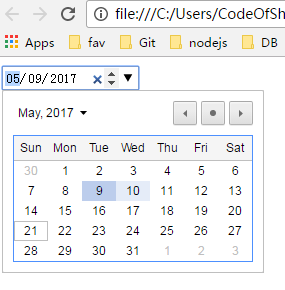
\includegraphics[width=5cm]{./img/h5_date.png}
                  \caption{H5 的日期输入表单}
                  \label{fig:h5_date}
                \end{figure}

                这些输入框还支持占位文本,一些网站的的输入框中一般会有提示字符,如图,这是通过 input 标签的 placeholder属性设置的,如图 \ref{fig:h5_placeholder}
                \begin{figure}[H]
                  \centering
                  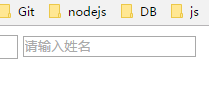
\includegraphics[width=5cm]{./img/h5_placeholder.png}
                  \caption{H 5 的占位文本}
                  \label{fig:h5_placeholder}
                \end{figure}
                当然,H5 还有很多特性,这里不一一列举。

        \subsection{CSS 3}
          \label{subsec:css_3}
            CSS 3 是最新的 CSS 标准,新增了丰富而强大的功能,圆角边框、颜色渐变、弹性盒子、动画等,我的项目中主要采用了圆角边框的特性。圆角边框看起来很美观,实现起来也很简单,常见于一些搜索框,如图 \ref{fig:h5_borderradius}。
            \begin{figure}[H]
              \centering
              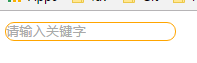
\includegraphics[width=5cm]{./img/h5_borderradius.png}
              \caption{圆角边框特性}
              \label{fig:h5_borderradius}
            \end{figure}

        \subsection{ES 5 和 ES 6}
          \label{subsubsec:es_5_和_es_6}
            \ref{subsubsec:javascript} 一节简要介绍了 JavaScript,我们知道 ECMAScript 是 JavaScript 的标准版本,简称 ES,目前的最新版是 ES6, 2015 年推出,也称 ES2015,但还未大量应用,目前的大部分框架仍是采用上个 ES 版本——ES5。ES 6 相比于 ES5添加了很多特性,比如支持显式地构造类,多了 class 关键词;有了块级作用域与 let 关键字;增加了遍历数组值的语法:of 关键字;增加了强大的 Generator 函数,让异步代码的书写更加容易,也可以用于构造"无限"数列, 这里的无限并不是一次性产生整个数列,而是可以放在循环中,按需要产生。
            \par
            新标准的诞生意味着框架的大规模更新,前端框架如 Angular2 ,基于 Nodejs 的后端框架如 KOA(Express 的下一代)。前端领域发展迅速,我们要顺应时代潮流,不断学习新技术。

        \subsection{前端库与框架,MVC}
          \label{subsec:前端库与框架}
            直接用 HTML,CSS,和 JavaScript 三种技术就可以开发网页。不过,如果要开发大型的应用,会非常难维护,代码量也会很巨大,因此,随着技术的发展,前端领域诞生了大量的库和框架,让开发应用更迅速,也更易维护,且大部分都是开源免费的,可以直接上 Github 上下载源码。那么什么是库,什么是框架呢?
            \par
            库是一些函数的集合,前端领域也包括样式库,如 Bootstrap, 提供了封装好了的一些常用功能,例如方便地设置漂亮的样式、动画,方便地获取与设置元素等,而且在一个项目中一般可以同时使用多个库,只要命名空间不重复即可。
            \par
            框架的使用直接影响到整个项目的架构。一个框架规范了整个项目的布局结构,提供了更高层次的抽象,也有了更多的概念。我们如果只开发一个十分简单的应用,项目结构完全可以由 img 文件夹、css 文件夹, js 文件夹和一些 html 文件构成,这样的设计只是根据文件的类型来划分的,没有所谓的抽象与概念,而如果采用框架来开发,项目结构就要遵循框架的规范,一个项目只能引入一个框架,而且有了众多的概念,例如:模板、控制器等,而且一个框架中可以引入多个库。
            \par
            目前主流的框架通常是基于 MVC 的,M(Module) 指的是模型,V(View) 是视图,C(Controller) 是控制器。模型一般负责数据库操作,控制器负责指挥分配,如:路由配置,为模板填充数据等,而视图就是 html 及其样式文件。这样划分项目的有很多的好处,数据、业务逻辑与模板视图分离,让代码更以维护。以往的动态网页会把代码逻辑与视图全部都写在一起,这样整个页面非常庞大,调试代码不好找,样式也不好控制,而数据与模型分开后,开发人员就可以更加专注,样式出问题了,就只管调样式,样式中没有逻辑,也好定位,同样,逻辑出了问题,只管调逻辑,而不用在意样式。
            \par
            但使用框架同样也有很多弊端,框架有很强的约束性,这要求我们要严格遵守,有时一个字母的大小写弄错都会出问题。出问题了不要紧,如果能很快定位到代码也可以,就怕定位不到代码,而是定位到上万行代码的框架中,这样就造成了调试的极度困难,只能对着文档一点点找错误,找不到还得在网上查阅大量资料,有时查阅大量资料还查不到,因为自己出现的问题很小,别人还没遇到,有时查到资料,但是怎么看也看不懂,因为不理解原理,这时又得花时间去学框架的原理,有时甚至要看源代码,而源代码很多地方又使用了很多高级的 JavaScript 功能,此时又得去花大量时间学习 JavaScript, 你看,就因为一个很小的问题,而花费了如此长的时间去修复,有时还修复不了,而且与其他库共用时也会产生问题。
            \par
            以上的问题在我的项目开发过程中我都遇到过,有时就是简单的几行代码,一旦出错,要花好久才找到,耽误了大量的时间,因此,用好框架是需要积累经验的,积累常见的错误,不可能短时间上手的。不过,这次的项目仍采用了框架 AngularJS, 我更多的关注了框架的优点,学习框架的理念,我相信用熟框架后可以大大提升开发速度。下面来介绍下本次项目用到的库与框架。

        \subsection{Bootstrap}
          \label{subsec:Bootstrap}
            Bootstrap 是一款非常优秀、广泛运用的一款前端库,是由 Twitter 的两位前员工 Mark Otto 和 Jacob Thornton 开发,在 2010 年 8 月面世。Bootstrap 总结了常见的样式与动画,可以快速搭建起网站,样式简洁、大气、美观,如图 \ref{fig:bootstrap}
            \begin{figure}[H]
              \centering
              
\includegraphics[width=10cm]{./img/bootstrap.png}
              \caption{简洁大方的 Bootstrap}
              \label{fig:bootstrap}
            \end{figure}

        \subsection{jQuery}
          \label{subsec:jquery}
            jQuery 是目前最流行的 JavaScript 库,2006 年 1 月 14 日诞生,作者为 John Resig。这是一个轻量的库,但功能强大。jQuery 有很多优秀的特性,几乎是前端开发必备的 JavaScript 库。我喜欢 jQuery 最主要的原因是它代码简洁,强大的 DOM 操作,还支持连缀、隐式遍历等功能。他的可以让我专注于功能,加快开发速度。我的项目的上个版本没有采用框架,全部都是用 jQuery 写的,但由于项目功能复杂,开发到最后实在难以维护,于是又换成了 AngularJS 框架,但有些地方仍在采用 jQuery ,因为 jQuery 的 DOM 操作是其他框架无法比拟的。

        \subsection{AngularJS}
          \label{subsec:angularjs}
            AngularJS 是一款强大的前端框架,诞生于 2009 年,作者是 Misko Hevery 。AngularJS采用纯 JavaScript 开发,没有依赖其他的库。AngularJS 适用于构建单页应用(SPA, Single Page Application),同时也是一款 MVC 框架,MVC 在前面介绍过,见 \ref{subsec:前端库与框架}  即视图与逻辑分离的框架。AngularJS 也有自己的一些全新的概念,例如服务(Services),依赖注入(), 指令(directives),脏检查……。AngularJS 是一个功能很强大的框架,给构建应用提供了大量的解决方案,因此适合构建大型的应用,不过我的项目比较小,只用到了很少的一些 AngularJS 的知识,我下面就来简要介绍一下。
            \subsubsection{SPA}
              \label{subsubsec:spa}
                AngularJS 适用于开发单页面应用,即 SPA(Single Page Applicaiton),单页应用的特点可以简单的概括为:模板 + 路由。只需一个入口 html 文件引入页面的基本结构以及所有的资源,如图 \ref{fig:index},
                \begin{figure}[H]
                  \centering
                  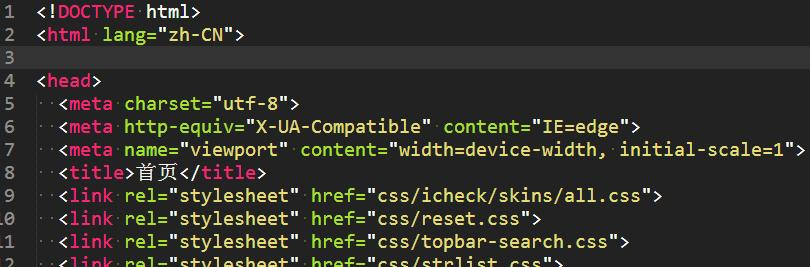
\includegraphics[width=10cm]{./img/index.jpg}
                  \caption{入口页示例}
                  \label{fig:index}
                \end{figure}

                其他的页面只需写入 html 片段即可, 如图 \ref{fig:tpl}

                \begin{figure}[H]
                  \centering
                  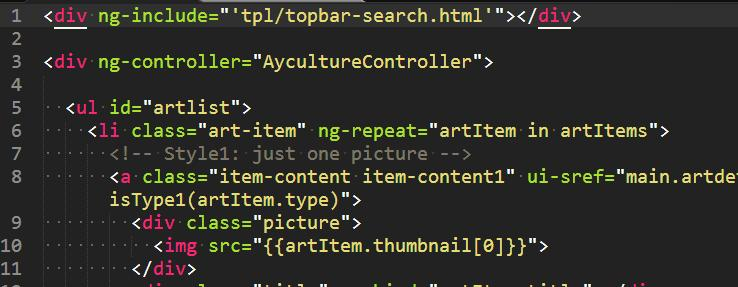
\includegraphics[width=10cm]{./img/tpl.jpg}
                  \caption{模板页示例}
                  \label{fig:tpl}
                \end{figure}

                路由的作用是:根据 url 控制加载相应的模板,通过 Angular 的 ui-router 模块实现,后面会具体讲解。如图 \ref{fig:router}

                \begin{figure}[H]
                  \centering
                  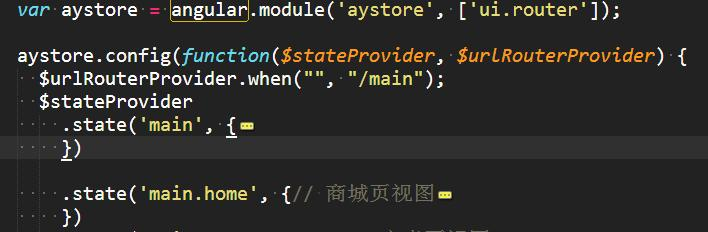
\includegraphics[width=10cm]{./img/router.jpg}
                  \caption{路由示例}
                  \label{fig:router}
                \end{figure}

            \subsubsection{控制器与模板引擎}
              \label{subsubsec:控制器与模板引擎}
                在没用 AngularJS 之前,如何向页面写入大量的数据对我来说是个非常棘手的问题,我之前是用的 jquery 实现的,利用了大量的 dom 操作和字符串拼接等,还利用了 h5 的 data-* 属性(防止引入过多的class或id),到最好实在难以维护,尤其是列表数据,如何让列表根据数据结构去展现是个比较麻烦的事情,如果用 jquery 实现的话,需要一个 for 循环,每个循环向模板中填充数据,填充数据的实现我也是靠 dom 操作,填充的数据包括标签的内容、标签的属性等,代码比较多,

                如图:reftodo,figtodo, jQuery 填充数据的复杂性

                才选择去使用一款框架的。
                \par
                AngularJS 没有让我失望,AngularJS 利用控制器去向模板中填入数据,每个控制器都有自己的域———\$scope, 只需把数据挂载到 \$scope 上,然后在模板中直接引入用双大括号括起来的变量名即可,非常方便。
                如图:AngularJs 的模板引擎
                而且,对于列表的形式, AngularJS 有独特的循环模板指令——ng-repeat, 写法类似于 Js 的 for...in 循环,十分方便,简化了大量的代码。

            \subsubsection{依赖注入}
              \label{subsubsec:依赖注入}
                调用控制器时,传入的第二个参数是一个回调函数,这个回调函数中可以根据需要加载相应的服务,不需要按照顺序,AngularJS 会根据参数名自动确定参数,这样就只需一个函数,不需要管他的参数,是一种神奇的机制。

            \subsubsection{ui-router 模块}
              \label{subsubsec:ui_router_模块}
                本项目采用了 AngularJS 的一个 ui-router 插件来配置路由。ui-router 的一个路由由一下几部分组成:
                \begin{itemize}
                  \item 状态名
                  \item url
                  \item 模板文件(html 文件的路径或字符串)
                  \item 各个视图
                  \begin{itemize}
                    \item 某个视图
                    \item 视图的模板
                  \end{itemize}
                \end{itemize}
                ui-router 的核心在于:子路由与多重视图。一个路由对应一个模板,而一个模板文件里面又有多个视图: ui-view, 每个视图又可以插入模板。子路由写法为:father.child, 子路由直接继承父路由的模板文件,然后可以修改父路由的部分视图,这就为模板的模块化提供了一种解决方案, ui-router 由图 \ref{fig:ui_view} 所示。
                \begin{figure}[H]
                  \centering
                  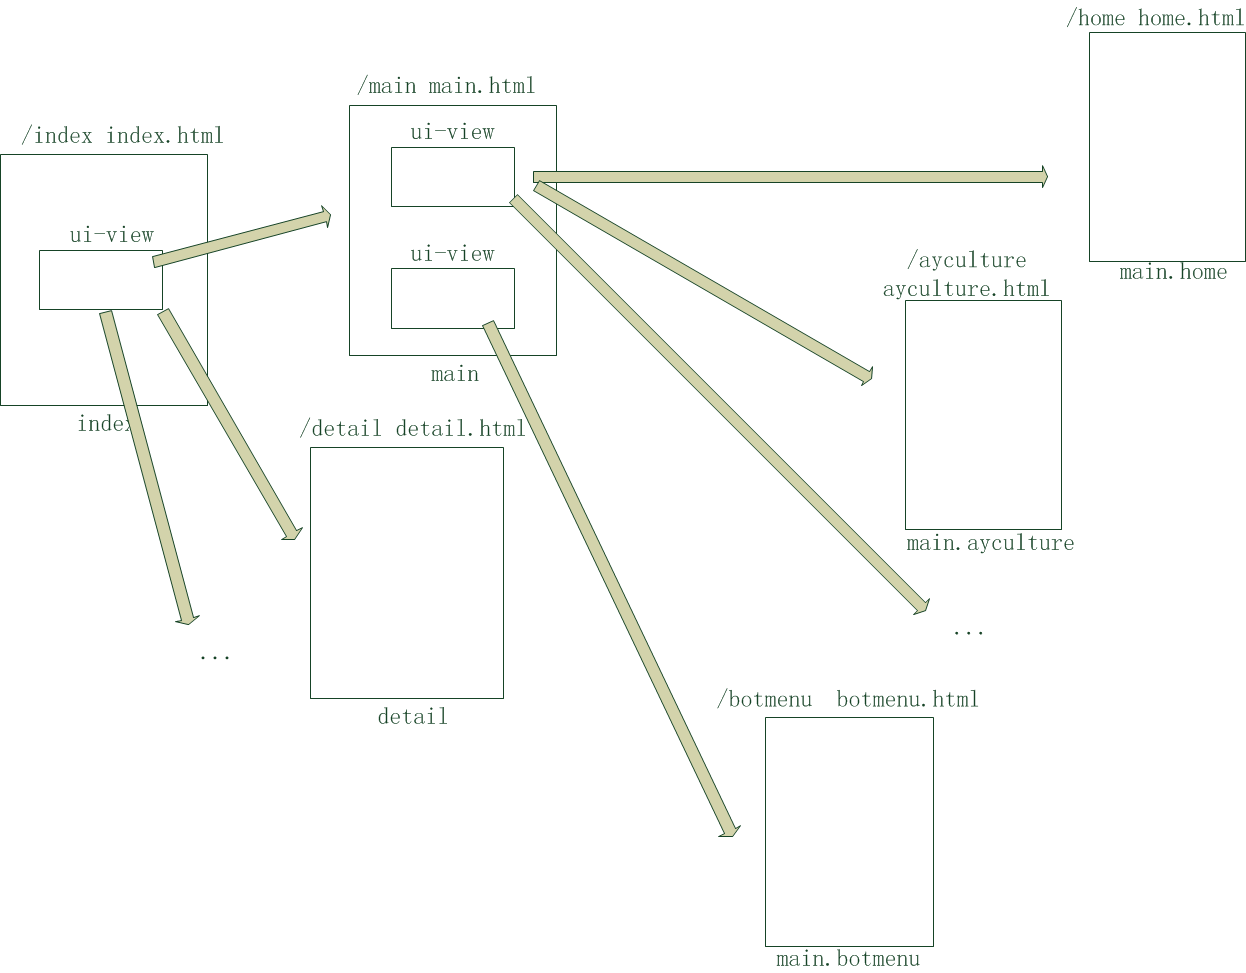
\includegraphics[width=12cm]{./img/ui_view.png}
                  \caption{ui-router 的示意图}
                  \label{fig:ui_view}
                \end{figure}
                项目的 9 个设计图中,有的页面有底部菜单,有的没有,因此就可以把有底部菜单的页面全都放在一个主路由下,项目路由的名称叫 main, 这些页面的路由只改变父路由的内容视图。其他的页面就每个单独配置路由即可。我把有底部菜单的页面全都配置成一个叫 "main" 路由的子路由,当URL跳转到这些页面时,这些页面的菜单部分不需要改动,只改动内容这个视图即可。

            \subsubsection{服务}
              \label{subsubsec:服务}
                AngularJS 的控制器有个特性,只会在需要的时候被实例化,而不需要时就会被销毁,每次切换路由或重新加载视图时,当前的控制器都会被 AngularJS 清除掉。而服务(Services)提供了一种在应用的整个生命周期保持数据的方法,能够在进程间通信。
                \par
                AngularJS 的服务分为两种,一种是内置服务,另一种是自定义服务。AngularJS 提供了一些内置服务,提供了一些常用的方法,例如
                \$timeout, \$http, \$factory等,我的项目中采用了 \$timeout 用于延时,这是为了解决 JS 异步加载的一个 bug,困扰了我好长时间;\$http 用于处理 http 请求,我的项目中需要向服务器请求商城列表、文章列表等,就会用到这个服务;\$factory 服务用来自定义服务,我的项目中自定了一个叫 DayAndTimeTest 的服务,用于根据艾灸服务的不同时段自动确定价格。

    \section{工具}
      \label{sec:工具}
        \subsection{Sublime Text 3}
          \label{subsec:sublime_text_3}
            Sublime Text 3 是一款非常强大的编辑器,如图 \ref{fig:sublime}, 目前是我最喜欢的编辑器,有诸多的优点:
            \paragraph{漂亮} Sublime 本身的字体就很美观,目前我换成了 Source Code Pro 字体,这是目前我认为最漂亮的字体。
            \begin{figure}[H]
              \centering
              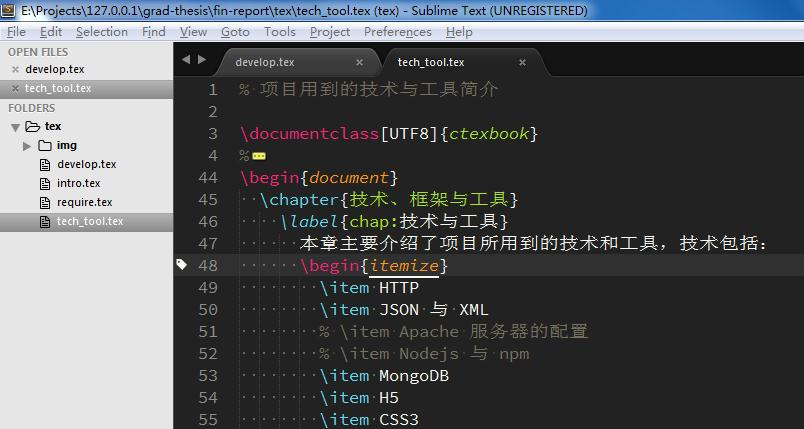
\includegraphics[width=10cm]{./img/sublime.jpg}
              \caption{Caption here}
              \label{fig:sublime}
            \end{figure}

            \paragraph{轻量} Sublime Text 3 的安装包只有 8 MB,即使在我安装了大量的插件(40 多个)后也不到 150MB,相比于 IDE 更加轻量,因此速度也是飞快。一个 IDE 至少几百兆甚至一两G, 大量的功能用不上,Sublime 的功能是根据需要来安装相应的插件,因此是按需索取,有更强的定制性。

            \paragraph{高效的操作} Sublime Text 官网中间就贴了一张动图,展示了 Sublime 的高效操作,如快速定位(文件、函数、某一行)、多光标编辑、快速选中单词和移动行等。

            \paragraph{插件系统、代码片段} Sublime 有着众多的插件,基本上可以打造任何编程语言的环境,语法高亮、实时纠错、代码片段等,让写代码快得飞起。

        \subsection{Chrome}
          \label{subsec:chrome}
            Chrome 是 Google 公司出品的浏览器,如图,
            \begin{figure}[H]
              \centering
              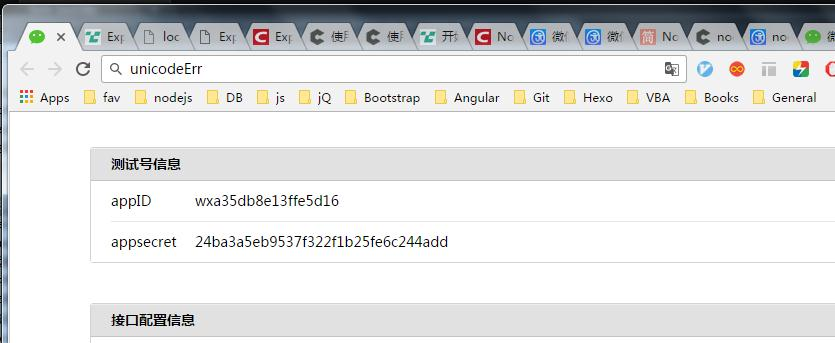
\includegraphics[width=10cm]{./img/chrome.jpg}
              \caption{Chrome 浏览器}
              \label{fig:chrome}
            \end{figure}
            功能强大,界面美观,兼容性好,有着强大的调试工具。Chrome 是前端开发必备的神器。浏览器的作用是渲染 HTML 和编译 JavaScript, HTML 在不断发展,不断增加新特性,这就要求浏览器的兼容性要好,同时 JavaScript 也在快速发展,浏览器此时作为编译引擎,性能要足够出色,Chrome 采用了 V8 引擎来编译 JavaScript ,是目前最快的编译引擎。同时,除了编译还要能够调试,Chrome 的调试功能也非常强大,如图 \ref{fig:chrome_debug}, 下面,我们就来详细谈谈 Chrome 的调试功能。
            \begin{figure}[H]
              \centering
              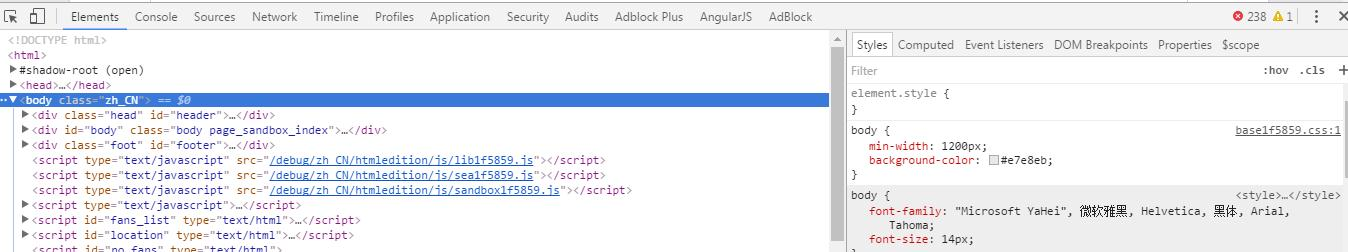
\includegraphics[width=12cm]{./img/chrome_debug.jpg}
              \caption{Chrome 的调试工具}
              \label{fig:chrome_debug}
            \end{figure}

            \subsubsection{Elements}
              \label{subsubsec:elements}
                我们看图 \ref{fig:chrome_debug} 中的几项菜单,第一个 Elements 是页面代码,可以方便的折叠和展开,坐上角的箭头一样的图标是用来审查(inspect)元素,如图 \ref{fig:cr_inspect},
                \begin{figure}[H]
                  \centering

                  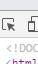
\includegraphics[width=2cm]{./img/cr_inspect.jpg}
                  \caption{Chrome 审查元素功能}
                  \label{fig:cr_inspect}
                \end{figure}
                翻译成捕捉更合适一点,因为它的功能是迅速定位元素在代码的位置,特别强大,如图 \ref{fig:cr_inspect1},
                \begin{figure}[H]
                  \centering
                  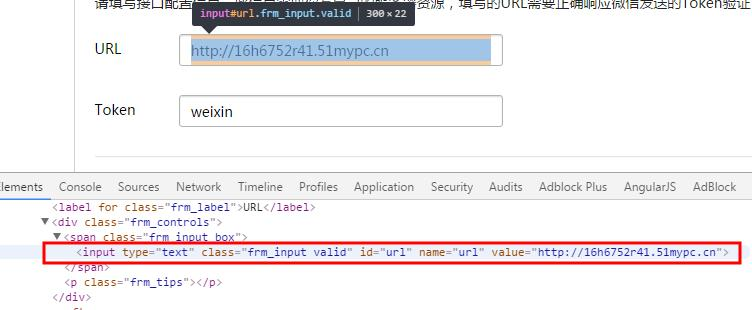
\includegraphics[width=10cm]{./img/cr_inspect1.jpg}
                  \caption{Chrome 定位元素的代码}
                  \label{fig:cr_inspect1}
                \end{figure}
                当点击审查元素的菜单后,我把鼠标移动到某个输入框上,Chrome 迅速为我定位到了其所在HTML代码处,同时右边还显示了对应的 CSS 样式,很强。
                \paragraph{title}
                \begin{figure}[H]
                  \centering
                  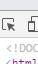
\includegraphics[width=3cm]{./img/cr_inspect.jpg}
                  \caption{Caption here}
                  \label{fig:figure1}
                \end{figure}

            \subsubsection{Console}
              \label{subsubsec:console}
                Console 即控制台,用于执行 javascript 语句和打印结果,如图 \ref{fig:cr_console},
                \begin{figure}[htbp]
                  \centering
                  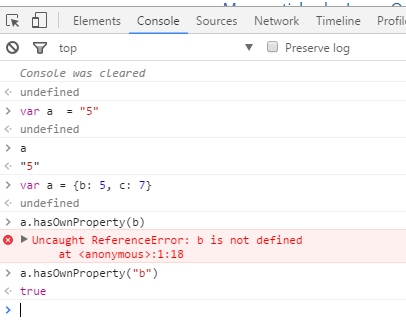
\includegraphics[width=8cm]{./img/cr_console.png}
                  \caption{控制台窗口}
                  \label{fig:cr_console}
                \end{figure}
                我一般用 Consolo 去测试一些 JavaScript 的方法、函数, dom 对象的一些方法以及测试 ajax 方法获取的数据是否正确。

            \subsubsection{Sources}
              \label{subsubsec:sources}
                Sources 是指加载的一些静态文件,如 html 文件,css 样式文件,图片,视频文件等,而加载的 js 文件可以进行断点调试,如图 \ref{fig:cr_sources}
                \begin{figure}[htbp]
                  \centering
                  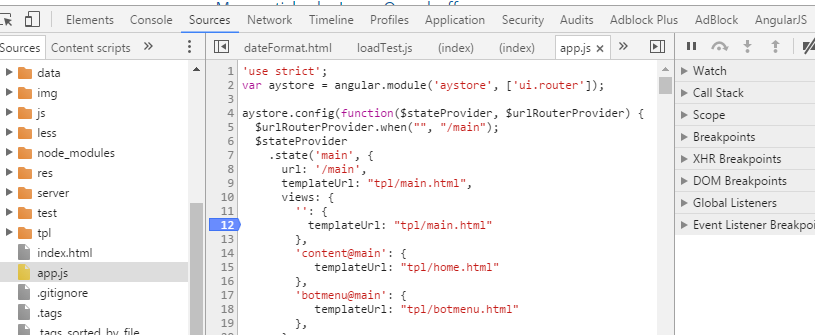
\includegraphics[width=10cm]{./img/cr_sources.png}
                  \caption{Sources}
                  \label{fig:cr_sources}
                \end{figure}
                变量的值还可以在当前执行的语句后显示出来。

            \subsubsection{Network}
              \label{subsubsec:network}



            \subsubsection{Application}
              \label{subsubsec:application}
                Application 一栏主要与缓存有关,如图 \ref{fig:cr_application}
                \begin{figure}[H]
                  \centering
                  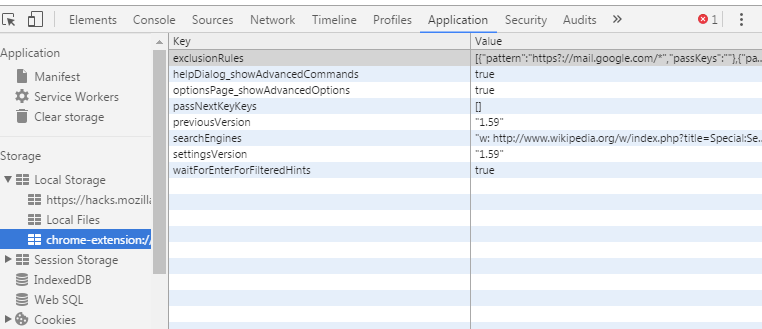
\includegraphics[width=10cm]{./img/cr_application.png}
                  \caption{application}
                  \label{fig:cr_application}
                \end{figure}
                左边 Application 目录下的 Manifest 保存了缓存文件的列表,Storage 目录下主要是本地存储技术,例如:
                \begin{itemize}
                  \item Local Storage
                  \item Session Storage
                  \item IndexedDB
                  \item WebSQL
                  \item Cookies
                \end{itemize}
                除了 Cookies,其他的存储方式都是 H5 新增的存储标准,容量一般都很大,例如 Local Storage 的容量可以达到 5MB, 而 Cookies 只有 4K,很多的网站开始尝试用 Local Storage 作为本地存储,而 IndexedDB 和 WebSQL 技术属于比较新的技术,还没有大面积使用。
                \par
                大量使用本地存储,对于服务器来说可以减轻负担,而对于客户端来说,减少了流量使用,提高了响应速度,Local Storage 我用来进行跨页数据传输问题,这只是方案之一,local Storage 的使用很方便,主要是 localStorage 对象,设置值用 localStorege.set('key', 'value') 或者 localStorege.key = value, 获取值用 localStorege.get('key') 或者 localStorege.key,因为 localStorage 也是一个对象,因此可以通过点或者中括号的方法获取或设置相应的值。
                \par
                以上介绍的功能是我在项目开发时常用的,调试非常方便,特别是在样式调试时的定位元素、实时修改属性值的时候,非常方便,而 JS 调试功能,如果是自己写的底层代码,即不用框架的话,调试起来是很方便的,会定位到相应的行,但是如果使用框架,问题就出来了,经常定位不到自己的代码中,而是定位到框架的代码中,如 angularjs 第 10500 行,此时就很头痛,只能把错误信息拿到网页去查询,这样的调试耗去了我大部分时间,针对框架调试的问题,我还没有找到好的方法。
                \par
                总之,Chrome 的调试工具无比强大,用好它可以大大缩短开发进度。

        \subsection{微信 Web 开发者工具}
          \label{subsec:微信_web_开发者工具}
            微信 Web 开发者工具是用来做微信开发的,实际上移动端的开发也可以用,如图 \ref{fig:wxweb}
            \begin{figure}[H]
              \centering
              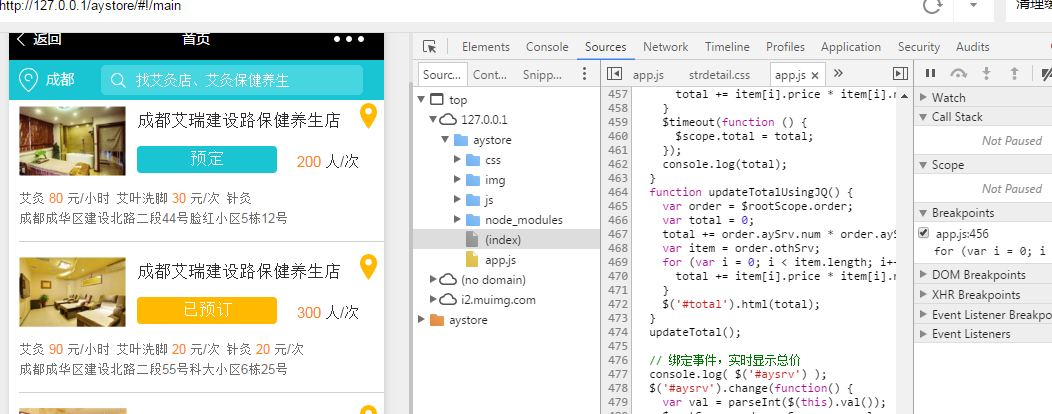
\includegraphics[width=10cm]{./img/wxweb.png}
              \caption{Caption here}
              \label{fig:wxweb}
            \end{figure}
            微信 Web 开发者工具采用的就是 Chrome 的调试工具,只不过只针对移动页面而已,不过也有其他的扩展,如 JSSDK 功能等。

        \subsection{Git}
          \label{subsec:git}
            Git 一款强大的版本控制工具,最早是用于 Linux 开发,由 Linux 系统的开发者 linus Trovals 研发。版本控制系统的目标是控制项目的版本,它可以记录你的每一次提交,因此你可以很方便的回到历史的版本,而不用去创建大量的备份,可以创建分支,团队协作开发等。Git 相对于其他的版本控制系统,更强大的地方在于本地仓库,每台设备都有一模一样的本地版本,不用担心中央服务器突然崩溃的问题。我个人用 Git 主要是用于版本同步,我有时在公司实习写的代码要和寝室的代码同步,简单的几行命令就可实现。

    \section{小结}
      \label{sec:小结}
        本章主要介绍了我在项目开发中用到的技术和工具,以上只是列举了我自己用得到的工具,事实上,前端领域中还有大量的工具,包括很多效果库、框架、自动化工具构建、测试工具等。工欲善其事必先利其器,工具用得好可以大大提升开发速度,简化重复的劳动,我们应该积极去学习,尤其是在前端这个发展迅猛的行业。


\end{document}

%  -- 技术与工具
  % %

\documentclass[UTF8]{ctexbook}

\ctexset{
    part/number = \chinese{part}% 用于解决 part 的标号不显示问题
}
\usepackage{hyperref}% 超链接
\hypersetup{
    colorlinks=false,% 去掉超链接颜色
    pdfborder=0 0 0% 取消超链接的边框
}
\usepackage{graphicx}% 图片管理
\graphicspath{{images/}}% 设置图片搜索路径
\usepackage{float,varwidth}% 浮动体
\usepackage{booktabs}% 三线表
\usepackage{tabularx}% 让表格自适应宽度与自动换行
\newcolumntype{Y}{>{\centering\arraybackslash}X}% 定义自适应列的居中格式 Y, 用 X 为左对齐(自适应列)
\usepackage{fancyhdr}% 页眉设置
\usepackage{xcolor}% 颜色宏包
\usepackage{listings}% 代码高亮
\definecolor{codegreen}{rgb}{0,0.6,0}
\definecolor{codegray}{rgb}{0.5,0.5,0.5}
\definecolor{codepurple}{rgb}{0.58,0,0.82}
\definecolor{backcolour}{rgb}{0.95,0.95,0.92}
\lstset{
    commentstyle=\color{codegreen},
    keywordstyle=\color{magenta},
    stringstyle=\color{codepurple},
    basicstyle=\footnotesize,% 代码字体大小
    breakatwhitespace=false,% 是否只在空白字符处断行
    breaklines=true,% 自动断行
    captionpos=b,% 标题位置为 bottom
    keepspaces=true,
    numbers=left,% 行号的位置
    numbersep=5pt,% 行号与代码的距离
    numberstyle=\tiny\color{codegray},% 行号样式
    stepnumber=2,% 隔行显示行号
    showspaces=false,
    showstringspaces=false,
    showtabs=false,
    tabsize=2
}

\begin{document}
  \chapter{开发流程}
    \label{chap:开发流程}

  \section{总体开发流程}
    \label{sec:总体开发流程}
      本次的项目采用 AngularJS 框架开发,AngularJS 项目一般由入口页、模板、控制器、路由控制以及静态资源几大模块构成。大体而流程是: 路由配置 -> 模板设计 -> 数据构造 -> 控制器配置,这些模块的编写没有严格的顺序,模块间是由关联的,因此,改动了一个模块,其他关联的而模块都要跟着改动,下面就简单介绍一下各流程所做的工作。

    \subsection{项目结构}
      \label{subsec:项目结构}
        整个项目的目录结构及如下:
                         aystore
                          |
                          |---css/ // CSS 静态资源
                          |    |---artdetail.css
                          |    |---artlist.css
                          |    |---botbar.css
                          |    ...
                          |
                          |---img/ // 主要是一些图标
                          |    |---alipay.png
                          |    |---home.jpg
                          |    ...
                          |
                          |---less // less 文件,用于编译成 CSS
                          |---node_modules // 项目用到的模块, 如 AngularJS
                          |---res // 存放一些资料,如设计图,方案规划等,不属于项目
                          |---tpl // 模板文件
                          |    |---artdetail.html
                          |    |---ayculture.html
                          |    |---pay.html
                          |    ...
                          |---app.js   // 控制器入口,路由控制,控制器代码
                          |---index.js // 视图入口,html 基本结构,静态资源的一次性引入
        \par
        css 目录是样式目录,用来控制页面的样式;img 目录放置了 html 文件中用到的所有的图标;less 目录是存放的 less 文件,要编译成 css 文件才能执行,我采用了 Sublime 的一个插件 Less2Css,使用时他会调用 lessc 引擎,在 Less 文件保存时可以自动将其编译为 css 文件到指定目录,非常高效。node_modules 文件夹存放了项目所需的库,由 npm 包管理工具下载的库或框架都放在 node_modules 文件夹下。res 文件夹存放了资料,例如项目规划、设计图等,不属于项目组成;tpl 文件夹存放了模板文件,对应于 MVC 模型中的 view, 由控制器控制路由与填充数据。入口页 index.html 负责引入页面的基本框架、静态资源以及视图入口。这是 SPA 应用的模式,详见 \ref{subsubsec:spa}。app.js 是控制逻辑的入口页,包含了路由的配置及各个模板的控制器。

    \subsection{路由配置}
      \label{subsec:路由配置}
        \begin{lstlisting}
            $stateProvider
              .state('main', {
                url: '/main',
                templateUrl: "tpl/main.html",
                views: {
                  '': {
                    templateUrl: "tpl/main.html"
                  },
                  'content@main': {
                     templateUrl: "tpl/home.html"
                  },
                  'botmenu@main': {
                     templateUrl: "tpl/botmenu.html"
                  },
                }
              })
          \end{lstlisting}
          上面的代码是主路由(或者叫父路由)的配置,state() 方法的第一个参数为状态名,或者叫路由名; 第二个参数是一个对象,url 字段表示 "main" 这个路由的路径,templateUrl 表示显示的页面文件,此页面文件的作用是划分视图,这里划分为两个视图,一个对应主要内容,另一个对应底部菜单

    \subsection{模板与样式设计}
      \label{subsec:模板与样式设计}
        一个模板就是一个页面,只不过很简洁,只有关键的 html 代码,而没有外部文件引入、页面头的设置等,如图 \ref{fig:tpl1}, 这就是前面提到的 SPA (单页应用)的特性,详见 \ref{subsubsec:spa} 一节。
        \begin{figure}[H]
          \centering
          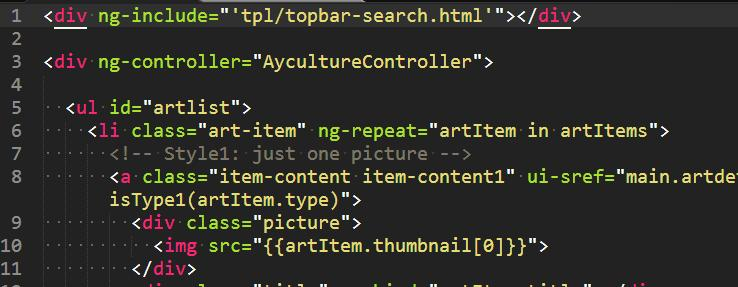
\includegraphics[width=8cm]{./img/tpl.jpg}
          \caption{简洁的模板页}
          \label{fig:tpl1}
        \end{figure}
        模板的主要作用是展现页面,因此要和配合 CSS 的控制。SPA 应用的样式需要考虑命名空间的问题,因为所有的 CSS 文件都是一次性引入的,如图 \ref{fig:css}
        \begin{figure}[H]
          \centering
          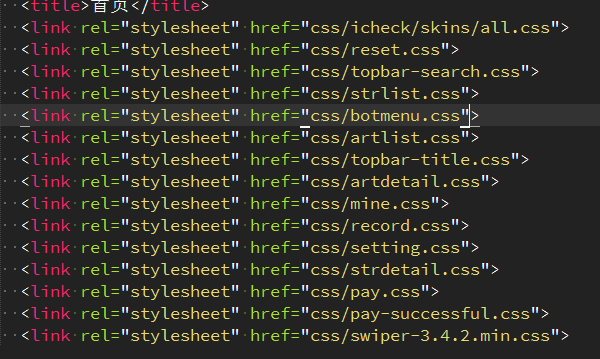
\includegraphics[width=10cm]{./img/css.png}
          \caption{一次性引入所有的 CSS 样式}
          \label{fig:css}
        \end{figure}
        我个人的处理方法是:对于每个 CSS 文件,用一个和文件名一样的容器把样式包裹起来,当然,我直接编辑的仍是 Less 文件,像这样 \ref{fig:wrapper},而且用 ID 而不是 Class 来确保唯一性, 让每个CSS 有自己的作用域,这个灵感来自于 AngularJS 的控制器的作用域,把每个模板的数据封闭起来,很好的避免了冲突。
        \begin{figure}[H]
          \centering
          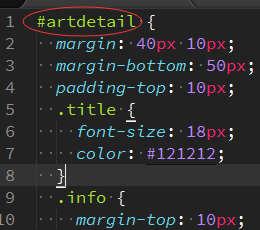
\includegraphics[width=5cm]{./img/wrapper.png}
          \caption{用 Wrapper 包裹起整个 Less 文件}
          \label{fig:wrapper}
        \end{figure}

    \subsection{数据构造}
      \label{subsec:数据构造}
        数据构造是前端设计中很重要的一环,个人认为,前端的设计大体分为两大块内容,一个是样式的设计,一个是数据的设计。好的样式设计需要花很长的时间,因为应用越精美,需要调的细节就越多;而数据部分,更多地涉及逻辑,属于 JavaScript 部分,这就需要开发者有着很强的 JavaScript 语言基础,尤其是 DOM 和 BOM 对象,掌握一门语言是要花很长时间的,大量的而应用才能更深入的理解本质,例如 JavaScript 的一些核心概念:原型、继承、对象等,如果理解不够深入,编写的代码就可能冗杂、难以维护。


    \subsection{控制器设计}
      \label{subsec:控制器设计}

      \par
      以上的步骤没有严格而顺序,因为各部分会相互关联,例如:修改模板的 HTML 结构时,样式文件也要跟着修改很多,因此,各个过程几乎是同时进行的。接下来我就对每一页的技术与设计过程进行详细介绍。

  \section{home 页的设计}
    \label{sec:home_页的设计}

    \subsection{功能分析}
      \label{subsec:功能分析}
      首页的设计图如下图所示:
      \begin{figure}[H]
        \centering
        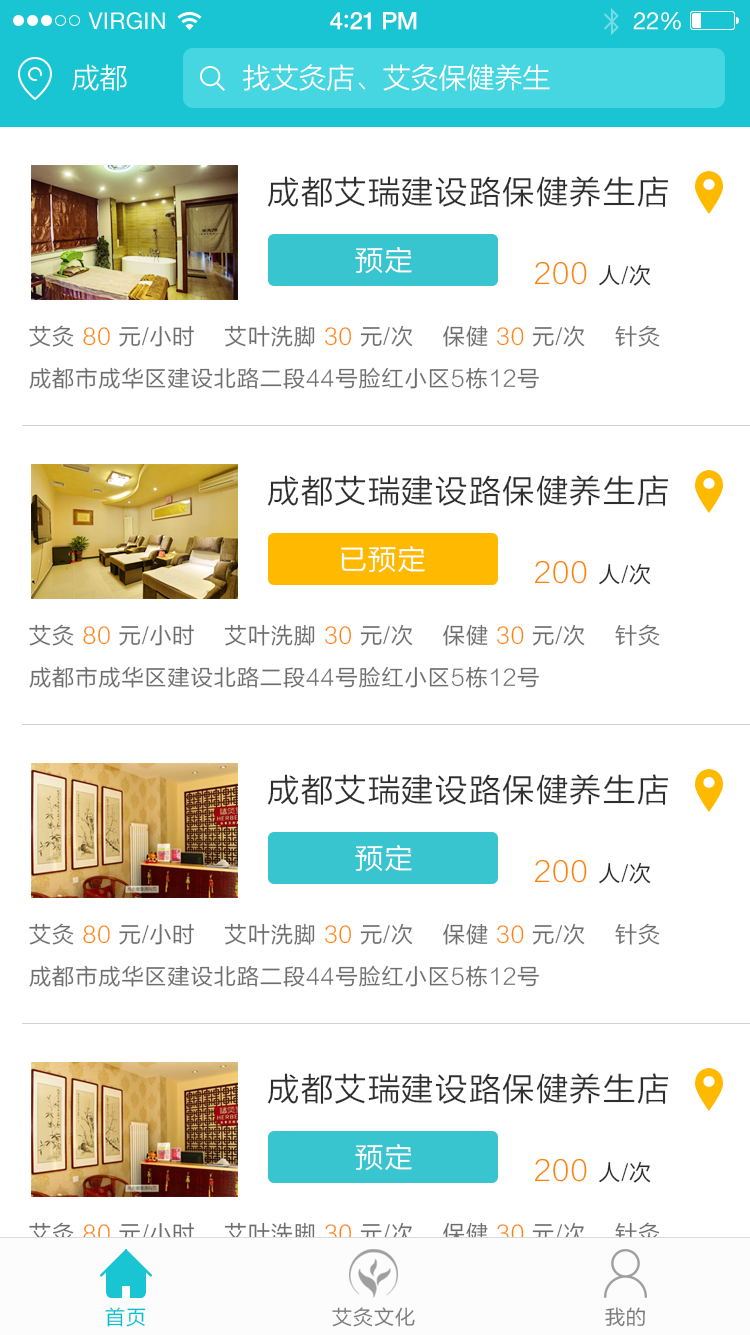
\includegraphics[width=8cm]{img/201705181050.jpg}
        \caption{首页设计图}
        \label{fig:home}
      \end{figure}
      首页主要实现如下功能:
      \begin{itemize}
        \item 地理定位
        \item 商城列表展现
        \item 商城搜索
      \end{itemize}

      \subsubsection{地理定位}
        \label{subsubsec:地理定位功能}
        首次进入商城,(todo)微信接口?还是自己写?应用会自动调用地理定位接口获取客户客户当前的位置,精确到县级,如:成华区,如果定位失败,则返回错误信息,位置自动设置为上一次的位置,并且提醒客户手动定位,点击左上方的按钮
        figtodo: 圈住左上方地理位置选择的图
        就会进入城市选择页,如下图所示:
        figtodo: 城市选择页
        然后就可以选择相应的城市或县区,为了更好地用户体验,如图,还设置了热门城市、最近选择的栏目。

      \subsubsection{列表展现}
        \label{subsubsec:列表展现}
        自动定位(或手动定位)好当前位置后,服务器会返回当前城市的保健店的列表,如图 todo 首页的设计图,简要地展示每个保健店的基本信息,如:店名、缩略图、艾灸床保健价格、其他服务与价格、详细地址以及右上角黄色的地理定位按钮,点击后会应用会打开地图接口,提供更好地体验,如下图:
        figtodo: 店的地图接口
        还有,如果一个店曾经预定过,则会以黄色的按钮提示已预订,点击预定按钮后就会进入店的详情页,展示店的详细信息以及进行预定操作。

      \subsection{商城搜索 todo: 待实现}
        \label{subsec:商城搜索_todo_待实现}
        如图figtodo: 首页设计图,还提供了搜索框,可以根据关键词搜索你想要的店,可以看到搜索框旁边没有搜索按钮,因为搜索是实时显示的,称为增量搜索,而且还采用了自动补全技术,根据最近的搜索关键词和列表加载时自动生成的关键词数据库进行模糊匹配,效果如下:设计非常人性化。
        figtodo: 搜索功能展示

    \subsection{地理定位功能 todo}
      \label{subsec:地理定位功能_todo}

    \subsection{搜索功能 todo}
      \label{subsec:搜索功能_todo}

    \subsection{列表展现}
      \label{subsec:列表展现}
      \subsubsection{数据设计}
        \label{subsubsec:数据设计}
        根据设计图 \ref{fig:home},列表中的每一项展示了如下的信息:
        \begin{itemize}
          \item 缩略图
          \item 店名
          \item 预定状态
          \item 艾灸保健价格
          \item 其他各项服务与价格
          \item 详细地址
        \end{itemize}
        于是我们可以构建如下的 JSON 数据,模拟从数据库提取的数据:
        \begin{lstlisting}
          [
              {
                "strId": "123",// 店的 ID
                "strCity": "成都",// 城市
                "strDistrict": "成华区",// 市区
                "strThumbnail": "http://i2.muimg.com/589268/8aefeb670174ad96t.jpg",// 缩略图
                "strName": "成都艾瑞建设路保健养生店",// 店名
                "ordStatus": 0,// 预定状态,0:已预订,1:未预定
                "strLink": "strlink/store1.html",// todo
                "avgPrice": 200,// 艾灸服务价格
                "srvInfo": "专业技术服务提供服务,智能艾灸床 5 张,艾灸、刮痧、洗脚、按摩、保健、亚健康、养生。",// 描述
                "full": 0,// 是否满员
                // 其他服务的信息
                "strServices": [
                  {
                    "srvName": "艾灸",// 服务名
                    "srvPrice": 80,// 服务价格
                    "srvUnit": "元/小时"// 价格单位
                  },
                  {
                    "srvName": "艾叶洗脚",
                    "srvPrice": 30,
                    "srvUnit": "元/次"
                  },
                  {
                    "srvName": "针灸",
                    "srvPrice": "",
                    "srvUnit": ""
                  }
                ],
                "strMap": "",// todo
                "strAddress": "建设北路二段44号脸红小区5栋12号"// 详细地址
              },
              {
                  "strId": "123",
                  "strCity": "成都",
                  "strDistrict": "成华区",
                  ...
              },
              ...
          ]
        \end{lstlisting}
        缩略图字段是调用的外部的链接,我把图片放到了专门的图片服务器上存储,这样可以节约服务器的空间,这样服务器上不需要再单独开辟一个文件夹盛放图片,也省去了给图片命名的麻烦,也能防止误删、图片文件夹改名的操作导致的图片链接失效。我采用的图片服务器是 “贴图库”,网址为:\url{http://www.tietuku.com/}, 网站虽然样式粗糙,但功能上考虑地很周到,例如可以给图片分组,方便管理,而且可以一键生成图片外链(包括缩略图),点击相应的按钮即可,如图:
        \begin{figure}[H]
          \centering
          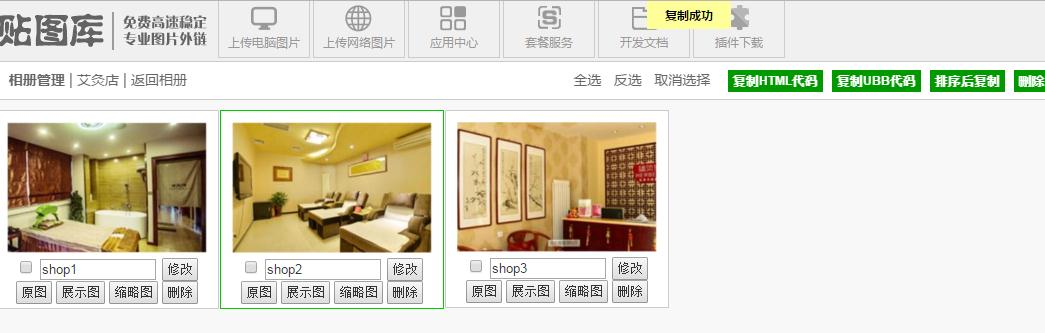
\includegraphics[width=10cm]{./img/tietuku.jpg}
          \caption{贴图库}
          \label{fig:tietuku}
        \end{figure}

      \subsubsection{dom 结构与 CSS 样式设计}
        \label{subsubsec:dom_结构与_css_样式设计}



      \subsubsection{控制器,路由}
        \label{subsubsec:控制器_路由}





















\end{document}
%    -- 开发流程
  % \chapter{成果展示}
  \label{chap:成果展示}
    本次的项目基本完成了商城前端部分的开发,功能演示如下。
    \section{商城模块}
      \label{sec:商城模块}
        商城页效果如图(\ref{fig:home_my}),
        \begin{figure}[htbp]
          \centering
          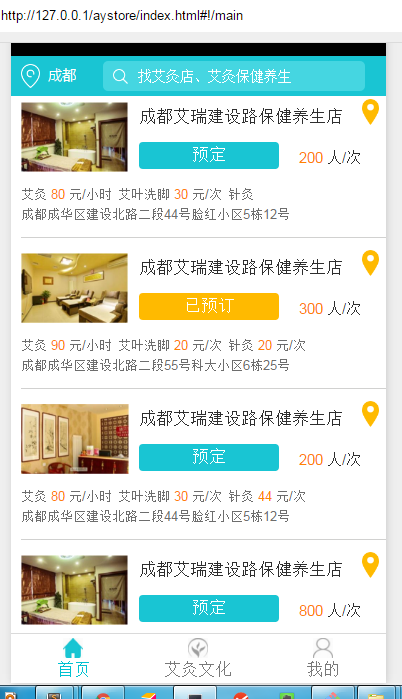
\includegraphics[width=5cm]{./img/home_my.png}
          \caption{商城页的效果展现}
          \label{fig:home_my}
        \end{figure}
        % \begin{figure}[htbp]
        %   \centering
        %   \subfigure[1]{
        %   \begin{minipage}{5cm}
        %     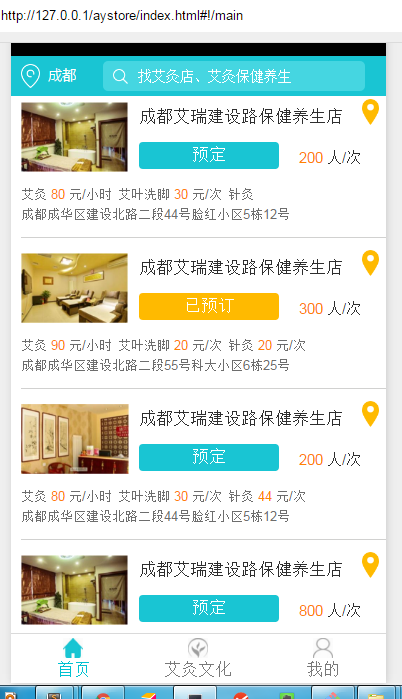
\includegraphics[width=5cm]{./img/home_my.png}
        %     \caption{商城页的效果展现}
        %     \label{fig:home_my}
        %   \end{minipage}
        %   }%
        %   \subfigure[1]{
        %   \begin{minipage}{5cm}
        %     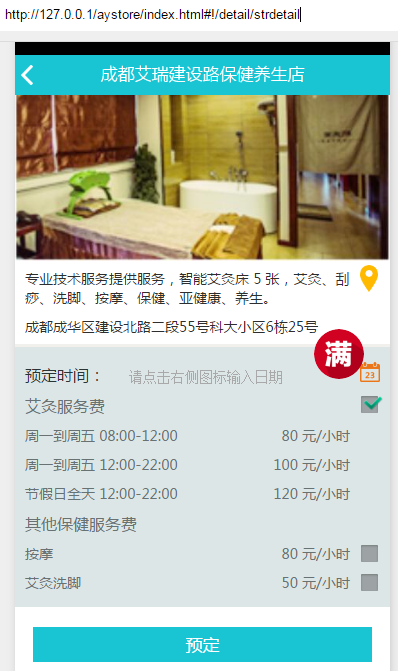
\includegraphics[width=5cm]{./img/strdetail_my.png}
        %     \caption{店铺详情的效果展现}
        %     \label{fig:strdetail_my}
        %   \end{minipage}
        %   }
        % \end{figure}
        这个页面上的数据不是静态的,而是通过 http 请求特定格式的 json 数据后填充的;店铺详情的效果如图(\ref{fig:strdetail_my}),
        \begin{figure}[htbp]
          \centering
          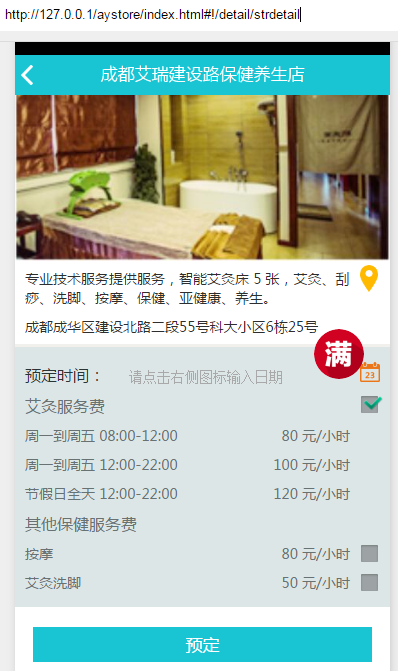
\includegraphics[width=5cm]{./img/strdetail_my.png}
          \caption{店铺详情的效果展现}
          \label{fig:strdetail_my}
        \end{figure}
        复选框的样式和设计图存在出入,设计图见(\ref{fig:strdetail_my}),但不影响基本功能,可以选择日期和时间,可以选择其他的服务。点击预定后进入下一页,可以继续选择人数等;支付页如图(\ref{fig:pay_my}),
        \begin{figure}[htbp]
          \centering
          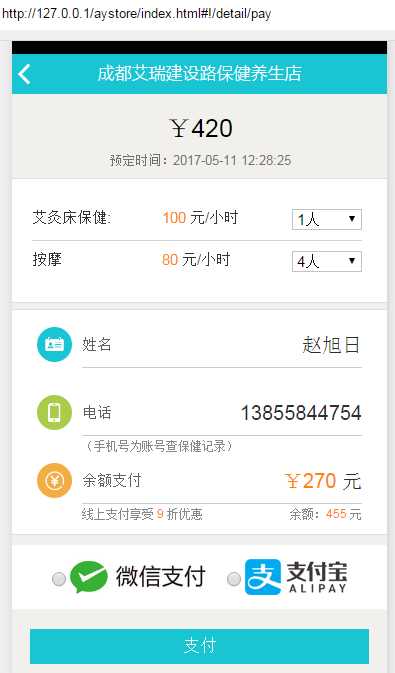
\includegraphics[width=5cm]{./img/pay_my.png}
          \caption{支付页的设计效果展现}
          \label{fig:pay_my}
        \end{figure}
        当选择人数时,上面可以实时现实总价;支付成功页如图(\ref{fig:pay_successful_my}),
        \begin{figure}[htbp]
          \centering
          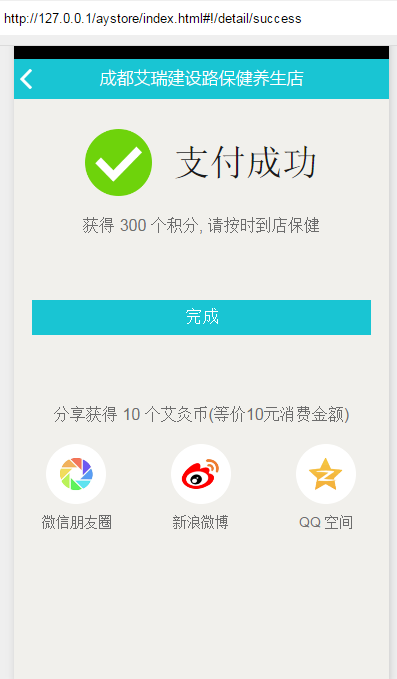
\includegraphics[width=5cm]{./img/pay_successful_my.png}
          \caption{支付成功页的设计效果展现}
          \label{fig:pay_successful_my}
        \end{figure}
        与设计图基本相符。

    \clearpage
    \section{文章模块}
      \label{sec:文章模块}
        文章列表页的效果如图(\ref{fig:artlist_my}),
        \begin{figure}[htbp]
          \centering
          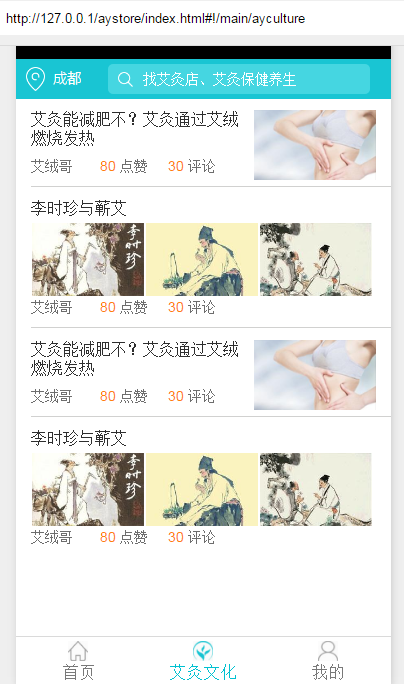
\includegraphics[width=5cm]{./img/artlist_my.png}
          \caption{文章列表页的效果展现}
          \label{fig:artlist_my}
        \end{figure}
        基本的信息都可以展示,这些数据也是通过 http 服务请求特定的数据而加载的,点击文章的任意一条后,跳转到文章详情页,如图(\ref{fig:artdetail_my}),
        \begin{figure}[htbp]
          \centering
          
\includegraphics[width=5cm]{./img/artdetail_my.png}
          \caption{文章详情页的效果展现}
          \label{fig:artdetail_my}
        \end{figure}
        点击收藏图标或喜欢图标后,图标会黄色,提示已经收藏或点赞,再次点击按钮又变为灰色。

    \clearpage
    \section{我的空间模块}
      \label{sec:我的空间模块}
        我的页效果如图(\ref{fig:mine_my}),
        \begin{figure}[htbp]
          \centering
          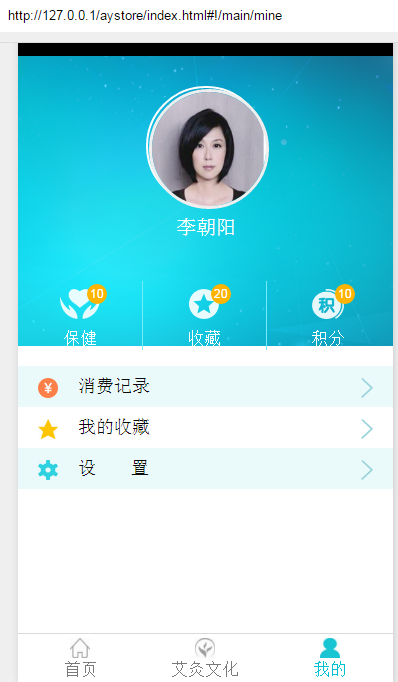
\includegraphics[width=5cm]{./img/mine_my.png}
          \caption{我的页效果展现}
          \label{fig:mine_my}
        \end{figure}
        点击消费记录一栏会进入消费记录页,如图(\ref{fig:record_my}),
        \begin{figure}[htbp]
          \centering
          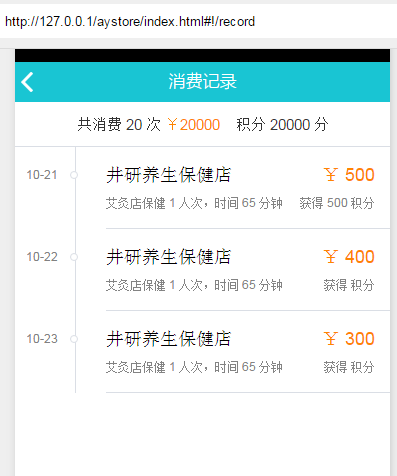
\includegraphics[width=5cm]{./img/record_my.png}
          \caption{消费记录页的效果展现}
          \label{fig:record_my}
        \end{figure}
        返回后,点击设置一栏会进入设置页,如图(\ref{fig:setting_my})。
        \begin{figure}[htbp]
          \centering
          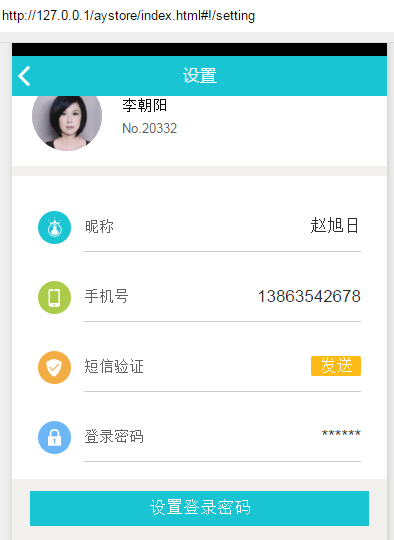
\includegraphics[width=5cm]{./img/setting_my.png}
          \caption{设置页效果展现}
          \label{fig:setting_my}
        \end{figure}

    \clearpage
    \section{本章小结}
      \label{sec:效果总结}
        以上我的项目目前所能实现的效果,不过还有很多功能未能实现,与理想的目标还有很长距离。
%    -- 成果
  % \chapter{结论}
  \label{chap:结论}
    观点和见解,归纳和总结
    本次商城的开发大体上完成了目标,尤其在样式的设计上投入了很多的精力,最终的样式效果与设计图几乎相符。
    本次项目的开发

\section{特色与意义}
  \label{sec:特色与意义}
    公众号运营,无需下载 App,直接关注公众号即可
    定制的商城,自己独立开发的一套框架,没有借用
    产品单一,
    技术新,此次的项目采用了强大的 AngularJS 框架开发,设计的应用代码量比较少,
    个人意义
    领域意义

\section{改进和完善}
  \label{sec:改进和完善}
    本次项目

\section{收获与感触}
  \label{sec:收获与感触}
  开发大型工程所注意的问题:多测试,模块化,熟练调试工具的使用
  学习方法:既要学又要练
  教训:理解原理很重要,
  大量学习
  框架与基础的思考:基础、原理很重要,学框架一定多探索背后的原理
    基础知识每天学,且时常复习
    每遇到遇到基础知识的问题,都要停下来测试
%    -- 结论 todo

  % 致谢

\thesisacknowledgement
  在项目开发中,很多人给了我帮助和支持。
  \par
  首先,我想感谢我的赖生建导师,我们导师有着丰富的开发经验,他注重从实践中学习,求真务实,学到的知识大量去实践,才能学得更深刻。他看中个人的主动学习能力,给你指明一个大体的方向,让你自己去找资料学习,这极大的培养了我的主动学习能力。
  \par
  在项目的开发中,我学到了大量的知识与经验,这部分主要来自于我看的书籍、慕课网的课堂、有道云课堂、youtube 上的一些教程以及大量博客文章,我非常感谢这些作者,教给我许多宝贵的经验。
  \par
  感谢我的同学们,在生活上给了我支持和鼓励。感谢黎承蕾同学,他对事物深刻的思考、喜欢探索本质的精神深深影响了我,让我在学习中更多地去思考,探究原理与本质。
%         -- 致谢
  % 参考文献

\begin{thesisbibliography}
  \bibitem{HTTP} 上野宣.图解 HTTP[M].于均良译.北京:人民邮电出版社, 2014.5
  \bibitem{HTML5} Pilgrim, M.HTML 5 揭秘[M].常可, 胡金埔, 赵静译.北京: 电子工业出版社, 2010.12
  \bibitem{CSS} Meyer, E.A.CSS 权威指南[M]: 第三版.尹志忠, 侯妍译.北京: 中国电力出版社, 2007.10
  \bibitem{AngularJS} Lerner, A.AngularJS 权威教程[M].赵望野, 徐飞, 何鹏飞译.北京: 人民邮电出版社, 2014.8
  \bibitem{jQuery} Chaffer, J, Swedberg, K.jQuery 基础教程: 第4版[M].李松峰译.北京: 人民邮电出版社, 2013.10
  \bibitem{OOJS} Stefanov, S.Object-Oriented JavaScript[M].Birmingham: Packt Publishing, 2008.7, 62-165
  \bibitem{NodeJS} 朴灵.深入浅出 NodeJS[M].北京: 人民邮电出版社, 2013.12
  \bibitem{less} Busy.less即学即用[OL].http://www.imooc.com/learn/102.
\end{thesisbibliography}

%            -- 参考文献
  % 附录

\thesisappendix
  \section{路由与部分控制器}
    \label{sec:控制器与路由部分}
      \begin{lstlisting}
        // 路由配置
        aystore.config(function($stateProvider, $urlRouterProvider) {
          $urlRouterProvider.when("", "/main");
          $stateProvider
            .state('main', {
              url: '/main',
              templateUrl: "tpl/main.html",
              views: {
                '': {
                  templateUrl: "tpl/main.html"
                },
                'content@main': {
                   templateUrl: "tpl/home.html"
                },
                'botmenu@main': {
                   templateUrl: "tpl/botmenu.html"
                },
              }
            })

            .state('main.home', {// 商城页视图
              url: '/home',
              views: {
                'content@main': {
                   templateUrl: "tpl/home.html"
                }
              }
            })
            .state('main.ayculture', {// 文章页视图
              url: '/ayculture',
              views: {
                'content@main': {
                   templateUrl: "tpl/ayculture.html"
                }
              }
            })
            .state('main.mine', {// 我的页视图
              url: '/mine',
              views: {
                'content@main': {
                   templateUrl: "tpl/mine.html"
                }
              }
            })

            .state('detail', {// 一些无底部菜单的页面
              url: '/detail',
              templateUrl: "tpl/detail.html"
            })
            .state('detail.strdetail', {// 商城详情页视图
              url: '/strdetail',
              templateUrl: "tpl/strdetail.html"
            })
            .state('detail.pay', {// 支付页视图
              url: '/pay',
              templateUrl: "tpl/pay.html"
            })
            .state('detail.success', {// 支付成功视图
              url: '/success',
              templateUrl: "tpl/pay-successful.html"
            })
            .state('detail.fail', {// 支付失败视图
              url: '/fail',
              templateUrl: "tpl/fail.html"
            })

            .state('main.artdetail', {// 文章详情页视图,含底部菜单
              url: '/artdetail',
              views: {
                'content@main': {
                   templateUrl: "tpl/artdetail.html"
                }
              }
            })

            .state('record', {// 消费记录页视图
              url: '/record',
              templateUrl: "tpl/record.html"
            })
            .state('collection', {// 收藏记录页视图
              url: '/collection',
              templateUrl: "tpl/collection.html"
            })
            .state('setting', {// 设置页视图
              url: '/setting',
              templateUrl: "tpl/setting.html"
            });
        });
        // 日期与时间判断服务
        aystore.factory('DayAndTimeTest', function(){
          var service = {};
          Array.prototype.contains = function(obj) {
            var i = this.length;
            while (i--) {
              if (this[i] === obj) {
                return true;
              }
            }
            return false;
          };

          function nthMinute(time) {
            var time = (time+"").replace(/ /gi, "");// 去空格
            var arr = time.split(":");
            var h = parseInt(arr[0]);
            var m = parseInt(arr[1]);
            return 60*h + m;
          }

          service.nthMinute = nthMinute;

          service.isDayInRange = function (date, range) {
            var day = new Date(date).getDay();
            day = (day === 0) ? 7 : day;
            range = range.replace(/ /gi, ""); // 去空格,如:"ff,  f, d ,f " -> "ff,f,d,f"
            var arr = [];
            var arr1 = range.split(",");
            var beg = 0;
            var end = 0;
            var item = "";
            for (let i=0; i<arr1.length; i++) {
              item = arr1[i];
              if (/-/.test(item)) {
                beg = parseInt(item.split("-")[0]);
                end = parseInt(item.split("-")[1]);
                while (beg <= end) {
                  arr.push(beg);
                  beg++;
                }
              } else {
                arr.push(parseInt(item));
              }
            }
            // console.log(day);
            // console.log(arr);
            // console.log(arr.contains(day));
            if (arr.contains(day)) {
              return true;
            } else {
              return false;
            }
          };

          service.isTimeInRange = function (time, range) {
            range = range.replace(/ /gi, "");
            var arr = range.split("-");
            var beg = nthMinute(arr[0]);
            var end = nthMinute(arr[1]);
            var time = nthMinute(time);
            return time >= beg && time <= end;
          };

          return service;
        });
        // 底部菜单状态控制
        aystore.controller('BotmenuController', function($scope, $state, $timeout) {
          // 初始化
          $scope.path1 = "img/home-selected.jpg";
          $scope.path2 = "img/ay.jpg";
          $scope.path3 = "img/mine.jpg";
          $scope.txtClass1 = 1;
          $scope.txtClass2 = 0;
          $scope.txtClass3 = 0;

          // 点击第一个按钮时的动作
          $scope.select1 = function() {
            $scope.path1 = "img/home-selected.jpg";
            $scope.path2 = "img/ay.jpg";
            $scope.path3 = "img/mine.jpg";
            $scope.txtClass1 = 1;
            $scope.txtClass2 = 0;
            $scope.txtClass3 = 0;
            // $timeout(function () {
            //   $state.go("home");
            // }, 100);

          };
          // 点击第二个按钮时的动作
          $scope.select2 = function() {
            $scope.path1 = "img/home.jpg";
            $scope.path2 = "img/ay-selected.jpg";
            $scope.path3 = "img/mine.jpg";
            $scope.txtClass1 = 0;
            $scope.txtClass2 = 1;
            $scope.txtClass3 = 0;
            // $timeout(function () {
            //   $state.go("ayculture");
            // }, 100);
          };
          // 点击第三个按钮时的动作
          $scope.select3 = function() {
            $scope.path1 = "img/home.jpg";
            $scope.path2 = "img/ay.jpg";
            $scope.path3 = "img/mine-selected.jpg";
            $scope.txtClass1 = 0;
            $scope.txtClass2 = 0;
            $scope.txtClass3 = 1;
            // $timeout(function () {
            //   $state.go("mine");
            // }, 100);
          };
        });

        // 艾灸店列表控制
        aystore.controller('HomeController', function($rootScope, $scope, $http) {
          $http.get('data/strlist.json', {
              params: {
                "custId": "12323",
                "data": "strList"
              },
              responseType: "json"
            })
            .then(function(res) {
              console.log(res.data.data);
              $rootScope.strItems = res.data.data;
            }, function() {
              alert('error');
            });
        });
        // 店铺详情
        aystore.controller('StrdetailController', function($rootScope, $scope, $http, $timeout, $state, DayAndTimeTest) {
          // 订单数据管理
          var order = {
            'ordId': 'adafdfefdvefsdvsd1213',
            'creTime': new Date().getTime(),
            'custId': 'sjdkfjsdfweioje12',
            'phone': 1234567,
            'srvTime': '',
            'aySrv': {
              'inputName': "ay",
              'name': '艾灸床保健',
              'price': 0,
              'num': 0
            },
            'othSrv': []
          };

          $http
            .get('data/strdetail.json', {
              params: {
                "custId": "12323",
                "data": "strdetail"
              },
              responseType: "json"
            })
            .then(function(res) {
              $rootScope.strdetail = res.data.data;
              $scope.strdetail = res.data.data;
              console.log($rootScope.strdetail);
              $rootScope.pageTitle = $rootScope.strdetail.strName;
            }, function() {
              alert('error');
            });
          // 日期选择插件
          $scope.setDate = function () {
            jeDate({
              dateCell: "#dateinput",
              format: "YYYY-MM-DD hh:mm:ss",
              isinitVal: true,
              isTime: true
            });
          };
          // 复选框插件
          $timeout(function () {
            $('input').iCheck({
               checkboxClass: 'icheckbox_polaris'
               // radioClass: 'iradio_polaris',
               // increaseArea: '-10' // optional
            });
          });

          function chooseService () {
            // 预定的保健时间
            order.srvTime = $('.sec-date input').val();
            // 根据预定时间判断艾灸服务的价格
            var date = order.srvTime.split(" ")[0];
            var day = new Date(date).getDay();// 星期几
            var time = order.srvTime.split(" ")[1];
            console.log("选择的日期:" + date + " 星期几:" + day);
            console.log("选择的时间:" + time);
            var aySrvPrice = $rootScope.strdetail.aySrvPrice;
            // console.log(aySrvPrice);
            var item = null;
            for (var i=0; i<aySrvPrice.length; i++) {
              item = aySrvPrice[i];
              console.log("");
              console.log(item.weekday + " " + item.srvTime);
              if (DayAndTimeTest.isDayInRange(day, item.weekday)) {
                console.log("日期在范围内");
                if (DayAndTimeTest.isTimeInRange(time, item.srvTime)) {
                  console.log("时间也在范围内");
                  order.aySrv.price = item.price;
                } else {
                  console.log("但时间不在范围内");
                }
              } else {
                console.log("日期不在范围内");
              }
            }
            if (order.aySrv.price === 0) {
              alert('日期不在规定范围内,请重新选择!');
              return;
            }
            // 主服务
            order.aySrv.num = $('.sec-aySrvPrice input').is(':checked') ? 1 : 0;

            // 其他服务的 post 数据构造
            var othSrvPrice = $rootScope.strdetail.othSrvPrice;
            $('.sec-othSrvPrice input').each(function(index, el) {
              if ($(this).is(':checked')) {
                order.othSrv.push({
                  'inputName': othSrvPrice[index].inputName,
                  'name': othSrvPrice[index].srvName,
                  'price': othSrvPrice[index].price,
                  'num': 1
                });
              }
            });

            // 必须选择一个服务
            console.log(order.aySrv.num === 0);
            console.log(order.othSrv.length === 0);
            if (order.aySrv.num === 0 && order.othSrv.length === 0) {
              alert("请至少选择一项服务");
              return;
            }

            console.log("订单数据:");
            console.log(order);
            $rootScope.order = order;
            $state.go('detail.pay');
          }

          $scope.chooseService = chooseService;

        });

        // 支付
        aystore.controller('PayController', function($rootScope, $scope, $timeout) {
          // 根据 order 的变动实时改变总价
          function updateTotal() {
            var order = $rootScope.order;
            var total = 0;
            total += order.aySrv.num * order.aySrv.price;
            var item = order.othSrv;
            for (var i = 0; i < item.length; i++) {
              total += item[i].price * item[i].num;
            }
            $timeout(function () {
              $scope.total = total;
            });
            console.log(total);
          }
          function updateTotalUsingJQ() {
            var order = $rootScope.order;
            var total = 0;
            total += order.aySrv.num * order.aySrv.price;
            var item = order.othSrv;
            for (var i = 0; i < item.length; i++) {
              total += item[i].price * item[i].num;
            }
            $('#total').html(total);
          }
          updateTotal();

          // 绑定事件,实时显示总价
          console.log( $('#aysrv') );
          $('#aysrv').change(function() {
            var val = parseInt($(this).val());
            $rootScope.order.aySrv.num = val;
            updateTotal();
          });

          $timeout(function () {
            console.log($('.part1').find('.othsrv'));
            $('.part1 select.othsrv').each(function (index, el) {
              $(this).change(function () {
                var val = parseInt($(this).val());
                console.log(val);
                $rootScope.order.othSrv[index].num = val;
                updateTotal();
              });
            });
          }, 1500);
        });
      \end{lstlisting}

  \section{部分模板文件}
    \label{sec:部分模板文件}
      \begin{lstlisting}
        // home.html
        <div ng-include="'tpl/topbar-search.html'"></div>

        <div ng-controller="HomeController">
          <ul class="strlist" id="strlist">
            <li class="store-item" ng-repeat="strItem in strItems">
              <div class="item-box">
                <div class="icon">
                  <img src="img/location-yellow.png" alt=""><!-- todo: 图标名字更换 -->
                </div>
                <div class="box-content clearfloat">
                  <img class="picture" ng-src="{{strItem.strThumbnail}}" alt="store picture">
                  <div class="name" ng-bind="strItem.strName"></div>
                  <div class="order clearfloat">
                    <a class="btn btn-small" ui-sref="detail.strdetail" ng-class="{0:'btn-blue', 1:'ordered'}[strItem.ordStatus]" ng-bind="{0:'预定', 1:'已预订'}[strItem.ordStatus]">
                    </a>
                    <span class="avg-price">
                      <span class="txt-number" ng-bind="strItem.avgPrice"></span> 人/次
                    </span>
                  </div>
                  <ul class="service">
                    <li ng-repeat="srvItem in strItem.strServices">
                      <span ng-bind="srvItem.srvName"></span>
                      <span ng-bind="srvItem.srvPrice" class="txt-number"></span>
                      <span ng-bind="srvItem.srvUnit"></span>
                    </li>
                  </ul>
                  <div class="address" ng-bind="strItem.strCity + strItem.strDistrict + strItem.strAddress"></div>
                </div>
              </div>
            </li>
          </ul>
        </div>
      \end{lstlisting}
      \begin{lstlisting}
        // strdetail.html
        <div ng-controller="StrdetailController">
          <div id="topbar-title">
            <a class="left-icon-back goback" onclick="goback()">
              <img src="img/back.png" alt="back.jpg">
            </a>
            <span class="name">{{pageTitle}}</span>
          </div>

          <div id="strdetail">
            <!-- banner 部分:店的大图 -->
            <section class="sec-banner">
              <div class="swiper-container">
                <div class="swiper-wrapper">
                  <div class="swiper-slide" ng-repeat="pic in strdetail.strPicture">
                    <img ng-src="{{pic}}" alt="">
                  </div>
                </div>
              </div>
            </section>

            <!-- intro 部分:店的简介部分 -->
            <section class="sec-intro store-info">
              <img class="icon" src="img/location-yellow.png" alt="">
              <p class="intro servie">{{strdetail.srvIntro}}</p>
              <p class="address">{{strdetail.strCity + strdetail.strDistrict + strdetail.strAddress}}</p>
            </section>
            <!-- 服务价格与选择 -->
            <section class="sec-order order-info3">
              <!-- 满员图标,根据返回的字段 full 设置其隐藏与否, 而求如果满的话,后面表单都无效,设为禁用状态 -->
              <div class="icon-full"></div>
              <!-- 日期时间选择 -->
              <section class="sec-date timepart clearfloat">
                <div class="icon">
                  <img class="" src="img/calendar.png" alt="" ng-click="setDate()">
                </div>
                <div class="title">预定时间:</div>
                <p class="datep time">
                  <input class="datainp" id="dateinput" type="text" placeholder="请点击右侧图标输入日期" readonly>
                </p>
                <!-- <img class="icon" src="img/calendar.png" alt=""> -->
              </section>

              <!-- 主服务 -->
              <section class="sec-aySrvPrice ayservicepart">
                <div class="title">
                  艾灸服务费
                  <input class="chk-aysrv checkbox" type="checkbox" name="aysrv" checked>
                </div>
                <ul class="">
                  <li class="clearfix" ng-repeat="aySrvItem in strdetail.aySrvPrice">
                    <div class="time">{{aySrvItem.weekdayDesc + "  " + aySrvItem.srvTime}}</div>
                    <div class="price">{{aySrvItem.price + "  " + aySrvItem.unit}}</div>
                  </li>
                </ul>
                <!-- <div class="icon checkbox1"></div> -->

                <!-- <input id="myothercheckbox" type="checkbox" class="icon checkbix" data-text="Checkbix. Large, checked" data-size="large"> -->
              </section>

              <!-- 其他服务 -->
              <setion class="sec-othSrvPrice othservicepart">
                <div class="title">
                  其他保健服务费

                </div>
                <ul>
                  <li class="clearfix" ng-repeat="othSrvItem in strdetail.othSrvPrice">
                    <div class="service">{{othSrvItem.srvName}}</div>
                    <div class="price">{{othSrvItem.price + " " + othSrvItem.unit}}</div>
                    <input class="chk-othsrv checkbox" type="checkbox" name="{{othSrvItem.inputName}}">
                  </li>
                </ul>
              </setion>
            </section>
            <a class="full btn btn-long btn-blue" data-full ng-click="chooseService()">
              预定
            </a>
          </div>
        </div>
      \end{lstlisting}

  \section{部分 Less 文件}
    \label{sec:部分_less_文件}
      \begin{lstlisting}
        // topbar-search.less
        #topbar-search {
          position: fixed;
          top: 0px;
          z-index: 1;
          width: 100%;
          height: 40px;
          font-family: "方正兰亭纤黑_GBK", "Microsoft YaHei", "serif";
          background-color: #19c5d3;
          .location-icon {
            position: absolute;
            top: 50%;
            left: 10px;
            height: 24px;
            margin-top: -12px;
            /*border: 1px solid #000;*/
            img {
              height: 100%;
            }
          }
          .location-text {
            margin-left: 37px;
            font-size: 14px;
            line-height: 40px;
            color: #fff;
          }
          .searchbox {
            position: absolute;
            left: 24.4%;
            top: 50%;
            width: 70%;
            height: 30px;
            margin-top: -15px;
            border-radius: 5px;
            background-image: url(../img/search.png);
            background-repeat: no-repeat;
            background-position: 10px center;
            background-size: 15px;
            background-color: #45d6e1;
            text-indent: 35px;
            font-size: 14px;
            border: none;
            &:focus {
              outline: none;
            }
            &::-webkit-input-placeholder {
              color: #fff;
            }
          }
        }
      \end{lstlisting}
      \begin{lstlisting}
        // strlist.less
        #strlist {
          margin-top: 30px;
          margin-bottom: 50px;
          width: 100%;
          background: #fff;
          .first {
            border-top: none !important;
            ;
          }
          .store-item {
            padding-left: 10px;
            .item-box {
              position: relative;
              padding-top: 15px;
              padding-bottom: 15px;
              padding-right: 25px;
              border-top: 1px solid #d1d1d0;
              .icon {
                position: absolute;
                top: 12px;
                right: 7px;
                height: 26px;
                img {
                  height: 100%;
                }
              }
              .box-content {
                .picture {
                  float: left;
                  height: 70px;
                  margin-bottom: 10px;
                  img {
                    height: 100%;
                  }
                }
                .name {
                  padding-top: 5px;
                  padding-left: 118px;
                  font-size: 17px;
                  color: #2e2e2e;
                }
                .order {
                  margin-top: 14px;
                  padding-left: 118px;
                  .btn {
                    width: 140px;
                  }
                  .avg-price {
                    display: inline-block;
                    float: right;
                    margin-top: 7px;
                    font-size: 15px;
                    color: #2e2e2e;
                  }
                }
                .service {
                  margin-top: 5px;
                  font-size: 13px;
                  color: #6d6d6d;
                  overflow: hidden;
                  text-overflow: ellipsis;
                  white-space: nowrap;
                  li {
                    float: left;
                    margin-right: 6px;
                  }
                }
                .address {
                  margin-top: 5px;
                  font-size: 13px;
                  color: #6d6d6d;
                }
              }
            }
          }
          .ordered {
            background-color: rgb(255, 186, 0);
            color: #fff;
          }
        }
      \end{lstlisting}






%       -- 附录
  % 英文资料原文

\thesistranslationoriginal
\section{ES6 In Depth: Generators}
  \label{sec:es6_in_depth_generators}
    \href{https://hacks.mozilla.org/category/es6-in-depth/}{ES6 In Depth} is a series on new features being added to the JavaScript programming language in the 6th Edition of the ECMAScript standard, ES6 for short.

    I'm excited about today's post. Today, we're going to discuss the most magical feature in ES6.

    What do I mean by "magical"? For starters, this feature is so different from things that already existed in JS that it may seem completely arcane at first. In a sense, it turns the normal behavior of the language inside out! If that's not magic, I don't know what is.

    Not only that: this feature's power to simplify code and straighten out "callback hell" borders on the supernatural.

    Am I laying it on a bit thick? Let's dive in and you can judge for yourself.

    \subsection{Introducing ES6 generators}
      \label{subsec:introducing_es6_generators}
        What are generators?

        Let's start by looking at one.

        \begin{lstlisting}
          function* quips(name) {
            yield "hello " + name + "!";
            yield "i hope you are enjoying the blog posts";
            if (name.startsWith("X")) {
              yield "it's cool how your name starts with X, " + name;
            }
            yield "see you later!";
          }
        \end{lstlisting}

        This is some code for a talking cat, possibly the most important kind of application on the Internet today. (Go ahead, click the link, play with the cat. When you're thoroughly confused, come back here for the explanation.)

        It looks sort of like a function, right? This is called a generator-function and it has a lot in common with functions. But you can see two differences right away:

        \begin{itemize}
          \item Regular functions start with function. Generator-functions start with function*.
          \item Inside a generator-function, yield is a keyword, with syntax rather like return. The difference is that while a function (even a generator-function) can only return once, a generator-function can yield any number of times. The yield expression suspends execution of the generator so it can be resumed again later.
        \end{itemize}

        So that's it, that's the big difference between regular functions and generator-functions. Regular functions can't pause themselves. Generator-functions can.

    \subsection{What generators do}
      \label{subsec:what_generators_do}
        What happens when you call the quips() generator-function?

        \begin{lstlisting}
          > var iter = quips("jorendorff");
            [object Generator]
          > iter.next()
            { value: "hello jorendorff!", done: false }
          > iter.next()
            { value: "i hope you are enjoying the blog posts", done: false }
          > iter.next()
            { value: "see you later!", done: false }
          > iter.next()
            { value: undefined, done: true }
        \end{lstlisting}

        You're probably very used to ordinary functions and how they behave. When you call them, they start running right away, and they run until they either return or throw. All this is second nature to any JS programmer.

        Calling a generator looks just the same: quips("jorendorff"). But when you call a generator, it doesn't start running yet. Instead, it returns a paused Generator object (called iter in the example above). You can think of this Generator object as a function call, frozen in time. Specifically, it's frozen right at the top of the generator-function, just before running its first line of code.

        Each time you call the Generator object's .next() method, the function call thaws itself out and runs until it reaches the next yield expression.

        That's why each time we called iter.next() above, we got a different string value. Those are the values produced by the yield expressions in the body of quips().

        On the last iter.next() call, we finally reached the end of the generator-function, so the .done field of the result is true. Reaching the end of a function is just like returning undefined, and that's why the .value field of the result is undefined.

        Now might be a good time to go back to the talking cat demo page and really play around with the code. Try putting a yield inside a loop. What happens?

        In technical terms, each time a generator yields, its stack frame—the local variables, arguments, temporary values, and the current position of execution within the generator body—is removed from the stack. However, the Generator object keeps a reference to (or copy of) this stack frame, so that a later .next() call can reactivate it and continue execution.

        It's worth pointing out that generators are not threads. In languages with threads, multiple pieces of code can run at the same time, usually leading to race conditions, nondeterminism, and sweet sweet performance. Generators are not like that at all. When a generator runs, it runs in the same thread as the caller. The order of execution is sequential and deterministic, and never concurrent. Unlike system threads, a generator is only ever suspended at points marked by yield in its body.

        All right. We know what generators are. We've seen a generator run, pause itself, then resume execution. Now for the big question. How could this weird ability possibly be useful?

    \subsection{Generators are iterators}
      \label{subsec:generators_are_iterators}
        Last week, we saw that ES6 iterators are not just a single built-in class. They're an extension point of the language. You can create your own iterators just by implementing two methods: [Symbol.iterator]() and .next().

        But implementing an interface is always at least a little work. Let's see what an iterator implementation looks like in practice. As an example, let's make a simple range iterator that simply counts up from one number to another, like an old-fashioned C for (;;) loop.

        \begin{lstlisting}
          // This should "ding" three times
          for (var value of range(0, 3)) {
            alert("Ding! at floor #" + value);
          }
        \end{lstlisting}

        Here's one solution, using an ES6 class. (If the class syntax is not completely clear, don't worry—we'll cover it in a future blog post.)

        \begin{lstlisting}
          class RangeIterator {
            constructor(start, stop) {
              this.value = start;
              this.stop = stop;
            }

            [Symbol.iterator]() { return this; }

            next() {
              var value = this.value;
              if (value < this.stop) {
                this.value++;
                return {done: false, value: value};
              } else {
                return {done: true, value: undefined};
              }
            }
          }

          // Return a new iterator that counts up from 'start' to 'stop'.
          function range(start, stop) {
            return new RangeIterator(start, stop);
          }
        \end{lstlisting}

        See this code in action.

        This is what implementing an iterator is like in Java or Swift. It's not so bad. But it's not exactly trivial either. Are there any bugs in this code? It's not easy to say. It looks nothing like the original for (;;) loop we are trying to emulate here: the iterator protocol forces us to dismantle the loop.

        At this point you might be feeling a little lukewarm toward iterators. They may be great to use, but they seem hard to implement.

        It probably wouldn't occur to you to suggest that we introduce a wild, mindbending new control flow structure to the JS language just to make iterators easier to build. But since we do have generators, can we use them here? Let's try it:

        \begin{lstlisting}
          function* range(start, stop) {
            for (var i = start; i < stop; i++)
              yield i;
          }
        \end{lstlisting}

        See this code in action.

        The above 4-line generator is a drop-in replacement for the previous 23-line implementation of range(), including the entire RangeIterator class. This is possible because generators are iterators. All generators have a built-in implementation of .next() and [Symbol.iterator](). You just write the looping behavior.

        Implementing iterators without generators is like being forced to write a long email entirely in the passive voice. When simply saying what you mean is not an option, what you end up saying instead can become quite convoluted. RangeIterator is long and weird because it has to describe the functionality of a loop without using loop syntax. Generators are the answer.

        How else can we use the ability of generators to act as iterators?

        \begin{itemize}
          \item Making any object iterable. Just write a generator-function that traverses this, yielding each value as it goes. Then install that generator-function as the [Symbol.iterator] method of the object.
          \item Simplifying array-building functions. Suppose you have a function that returns an array of results each time it's called, like this one:
        \end{itemize}

        \begin{lstlisting}
          // Divide the one-dimensional array 'icons'
          // into arrays of length 'rowLength'.
          function splitIntoRows(icons, rowLength) {
            var rows = [];
            for (var i = 0; i < icons.length; i += rowLength) {
              rows.push(icons.slice(i, i + rowLength));
            }
            return rows;
          }
        \end{lstlisting}

        Generators make this kind of code a bit shorter:

        \begin{lstlisting}
          function* splitIntoRows(icons, rowLength) {
            for (var i = 0; i < icons.length; i += rowLength) {
              yield icons.slice(i, i + rowLength);
            }
          }
        \end{lstlisting}

        The only difference in behavior is that instead of computing all the results at once and returning an array of them, this returns an iterator, and the results are computed one by one, on demand.

        \begin{itemize}
          \item Results of unusual size. You can't build an infinite array. But you can return a generator that generates an endless sequence, and each caller can draw from it however many values they need.
          \item Refactoring complex loops. Do you have a huge ugly function? Would you like to break it into two simpler parts? Generators are a new knife to add to your refactoring toolkit. When you're facing a complicated loop, you can factor out the part of the code that produces data, turning it into a separate generator-function. Then change the loop to say for (var data of myNewGenerator(args)).
          \item Tools for working with iterables. ES6 does not provide an extensive library for filtering, mapping, and generally hacking on arbitrary iterable data sets. But generators are great for building the tools you need with just a few lines of code. \\
          For example, suppose you need an equivalent of Array.prototype.filter that works on DOM NodeLists, not just Arrays. Piece of cake:\\
          \begin{lstlisting}
            function* filter(test, iterable) {
              for (var item of iterable) {
                if (test(item))
                  yield item;
              }
            }
          \end{lstlisting}
        \end{itemize}

        So are generators useful? Sure. They are an astonshingly easy way to implement custom iterators, and iterators are the new standard for data and loops throughout ES6.

        But that's not all generators can do. It may not even turn out to be the most important thing they do.

    \subsection{Generators and asynchronous code}
      \label{subsec:generators_and_asynchronous_code}
        Here is some JS code I wrote a while back.

        \begin{lstlisting}
                    };
                  })
                });
              });
            });
          });
        \end{lstlisting}

        Maybe you've seen something like this in your own code. Asynchronous APIs typically require a callback, which means writing an extra anonymous function every time you do something. So if you have a bit of code that does three things, rather than three lines of code, you're looking at three indentation levels of code.

        Here is some more JS code I've written:

        \begin{lstlisting}
          }).on('close', function () {
            done(undefined, undefined);
          }).on('error', function (error) {
            done(error);
          });
        \end{lstlisting}

        Asynchronous APIs have error-handling conventions rather than exceptions. Different APIs have different conventions. In most of them, errors are silently dropped by default. In some of them, even ordinary successful completion is dropped by default.

        Until now, these problems have simply been the price we pay for asynchronous programming. We have come to accept that asynchronous code just doesn't look as nice and simple as the corresponding synchronous code.

        Generators offer new hope that it doesn't have to be this way.

        Q.async() is an experimental attempt at using generators with promises to produce async code that resembles the corresponding synchronous code. For example:

        \begin{lstlisting}
          // Synchronous code to make some noise.
          function makeNoise() {
            shake();
            rattle();
            roll();
          }

          // Asynchronous code to make some noise.
          // Returns a Promise object that becomes resolved
          // when we're done making noise.
          function makeNoise_async() {
            return Q.async(function* () {
              yield shake_async();
              yield rattle_async();
              yield roll_async();
            });
          }
        \end{lstlisting}

        The main difference is that the asynchronous version must add the yield keyword each place where it calls an asynchronous function.

        Adding a wrinkle like an if statement or a try/catch block in the Q.async version is exactly like adding it to the plain synchronous version. Compared to other ways of writing async code, this feels a lot less like learning a whole new language.

        If you've gotten this far, you might enjoy James Long's very detailed post on this topic.

        So generators are pointing the way to a new asynchronous programming model that seems better suited to human brains. This work is ongoing. Among other things, better syntax might help. A proposal for async functions, building on both promises and generators, and taking inspiration from similar features in C\#, is on the table for ES7.

    \subsection{When can I use these crazy things?}
      \label{subsec:when_can_i_use_these_crazy_things_}
        On the server, you can use ES6 generators today in io.js (and in Node if you use the --harmony command-line option).

        In the browser, only Firefox 27+ and Chrome 39+ support ES6 generators so far. To use generators on the web today, you'll need to use Babel or Traceur to translate your ES6 code to Web-friendly ES5.

        A few shout-outs to deserving parties: Generators were first implemented in JS by Brendan Eich; his design closely followed Python generators which were inspired by Icon. They shipped in Firefox 2.0 back in 2006. The road to standardization was bumpy, and the syntax and behavior changed a bit along the way. ES6 generators were implemented in both Firefox and Chrome by compiler hacker Andy Wingo. This work was sponsored by Bloomberg.

        yield;

        There is more to say about generators. We didn't cover the .throw() and .return() methods, the optional argument to .next(), or the yield* expression syntax. But I think this post is long and bewildering enough for now. Like generators themselves, we should pause, and take up the rest another time.

        But next week, let's change gears a little. We've tackled two deep topics in a row here. Wouldn't it be great to talk about an ES6 feature that won't change your life? Something simple and obviously useful? Something that will make you smile? ES6 has a few of those too.

        Coming up: a feature that will plug right in to the kind of code you write every day. Please join us next week for a look at ES6 template strings in depth.
%   -- 英文资料原文
  % 英文资料译文

\thesistranslationchinese
\section{深入理解ES6: Generators}
  我的深入理解 ES6 系列文章简要讨论了 JavaScript 语言第六版————ESMAScript 6(缩写为 ES6)的新特性。

  今天写的文章让我很兴奋,因为我们将去讨论 ES6 最神奇的一些特性。

  我说的神奇是什么意思?对于初学者,这些特性和以往的 JS 有很大的不同,你第一次接触会感到很难理解。在某种程度上,这些特性完全颠覆了语言的行为!

  不仅仅是这些,这些强大的特性可以简化代码、让你看清可怕的"回调函数地狱"的界限。

  我的溢美之词是不是太多了?那我们开始吧。

  \subsection{ES6 Generators}
    \label{subsec:es6_generators}
      Generator 是什么?

      先来个例子吧。

      \begin{lstlisting}
        function* quips(name) {
          yield "hello " + name + "!";
          yield "i hope you are enjoying the blog posts";
          if (name.startsWith("X")) {
            yield "it's cool how your name starts with X, " + name;
          }
          yield "see you later!";
        }
      \end{lstlisting}

      这是一个"\href{http://people.mozilla.org/~jorendorff/demos/meow.html}{会说话的猫}"小例子的一些代码,这可能是今天互联网上最重要的一种应用。(你可以点击\href{http://people.mozilla.org/~jorendorff/demos/meow.html}{这个链接},玩一玩这只猫。当你困惑的时候,再回到这篇文章寻找解释。)

      看起来像函数,是吗?这个叫做生成器函数(generator-function), 和普通的函数有很多共同点。但你很快就能看出差别:

      \begin{itemize}
        \item 普通的函数以关键字 \keyword{function} 开头,而生成器函数(generator-function)以 \keyword{function*} 开头。
        \item 在 generator-function 中,\keyword{yield} 是关键字,语法上就像 \keyword{return}。不同点是虽然一个函数只能返回一次,但 generator-function 可以 yield 很多次。\keyword{yield} 关键字暂停了 generator 的执行,之后还可以继续往下执行。
      \end{itemize}

      就是这样,这就是普通的函数和 generator-function 最大的不同。普通的函数不能暂停,而 generator-function 就可以。

  \subsection{generators 是怎么执行的}
    \label{subsec:generators_是怎么执行的}

      当你调用 quips() 这个 generator-function 时候发生了什么?

      \begin{lstlisting}
        > var iter = quips("jorendorff");
          [object Generator]
        > iter.next()
          { value: "hello jorendorff!", done: false }
        > iter.next()
          { value: "i hope you are enjoying the blog posts", done: false }
        > iter.next()
          { value: "see you later!", done: false }
        > iter.next()
          { value: undefined, done: true }
      \end{lstlisting}

      你可能对普通的函数比较熟悉,知道他们怎么执行的。当你调用他们的时候,他们就立即执行,一直到他们返回或抛出异常。

      调用一个 generator 形式上看起来一样:\keyword{quips("jorendorrff")}。但当你调用 generator 的时候,他不会立即开始执行。相反,他返回一个 Generator 对象(上个例子中叫做 \keyword{iter})。你可以把这个 Generator 对象看成是函数调用,在 generator-function 执行第一段代码之前就会停住。

      之后你每次调用 Generator 对象的 \keyword{.next()} 方法,函数就会往下执行直到遇到下个 \keyword{yield}。

      这就是为什么每次我们每次调用上面的 \keyword{iter.next()}, 我们就会得到一个不同的字符串值。这些值是由 \keyword{yield} 产生的。

      最后一次 \keyword{iter.next()} 调用,终于执行到 generator-function 的最后,打印的对象的 \keyword{done} 字段由 \keyword{false} 变为 \keyword{true}, 而此时 \keyword{.value} 字段变为 \keyword{undefined}。

      现在是时候回到我们的"说话的猫"这个演示页面。如果把 \keyword{yield} 放进 loop 会怎样?

      在技术术语上,每次 generator yields, 他的栈结构(局部变量,参数,临时值,当前执行到的位置)会从栈中移出。但 Generator 对象保留着栈的引用,这样之后的 \keyword{.next()} 调用就可以重新继续执行。

      值得注意的是 Generators 不是线程。有线程的语言,多块代码可以同时运行,这样会导致资源竞争,不确定性以及性能问题。Generators 和这个不同。generator 执行时,执行是有确定的顺序的,不会并发。不像系统进程,generator 只会在 \keyword{yield}
      标记的地方暂停。

      我们现在知道了 generators 是什么了。我们知道 generator 执行的时候,暂停自己,然后再继续执行。那么问题又来了,这种奇怪的特性有什么呢?

  \subsection{Generators 是迭代器(iterators)}
    \label{subsec:generators_是迭代器_iterators_}
      上周,我们看到迭代器不仅仅是是个内置的类。是可以扩展的。你可以创建自己的迭代器,只需实现两个方法:: \keyword{[Symbol.iterator]()} and \keyword{.next()}。

      但去实现一个接口要花点时间。我们来看看一个 iterator 是如何实现的。先来看个例子,我们来写一个简单的 \keyword{range} iterator ,作用是从一个数字一直计数到另一个数字,类似于 \keyword{for(;;)} 循环。

      \begin{lstlisting}
        // This should "ding" three times
        for (var value of range(0, 3)) {
          alert("Ding! at floor #" + value);
        }
      \end{lstlisting}

      实现的一种方法是使用 ES6 的 class。(如果对 class 语法不是很清楚,别担心,我会在后面的文章讨论)。

      \begin{lstlisting}
        class RangeIterator {
          constructor(start, stop) {
            this.value = start;
            this.stop = stop;
          }

          [Symbol.iterator]() { return this; }

          next() {
            var value = this.value;
            if (value < this.stop) {
              this.value++;
              return {done: false, value: value};
            } else {
              return {done: true, value: undefined};
            }
          }
        }

        // Return a new iterator that counts up from 'start' to 'stop'.
        function range(start, stop) {
          return new RangeIterator(start, stop);
        }
      \end{lstlisting}

      这就是 iterator 的一种实现,类似于 Java 和 Swift 语言。这段代码有 bugs 吗? 不好说。看起来和 for(;;) 循环不像。iterator 的这种特性迫使我们拆开循环。

      现在你可能对 iterators 感到有点不爽了是吧。iterator 挺好用,但不好实现。

      在 JS 语言中引入一个新的令人费解的控制结构让 iterator 更容易实现,这种做法我们或许想不到。但既然我们有 generators, 我们可以使用它吗?试试看吧:

      \begin{lstlisting}
        function* range(start, stop) {
          for (var i = start; i < stop; i++)
            yield i;
        }
      \end{lstlisting}

      上面四行代码就是对上面的 23 行代码的一个简单的替代包括整个 RangeIterator class. 这可能是由于 generators 是 iterator 的缘故。所有的 generators 都有一个内置的 \keyword{.next()} 和 \keyword{[Symbol.iterator]} 。

      不用 generators 去实现 iterators 就像被迫全部用被动语态写一篇长的 email。RangeIterator 这个类的代码又长又奇怪,因为他必须描述一个循环而且还不能使用循环语法。Generators 就是很好的一个替代品。

      我们还可以怎样用 generator 的特性去实现 iterator ?

      \begin{itemize}
        \item 让任意的对象可迭代(iterable). 你就写一个 genertor-function 遍历 this 对象,每次用 yield 产生对应的值。再把 generator-function 安装为 [Symbol.iterator] 这个对象的方法。
        \item 简化构建数组的函数。假设你有个函数,每次被调用时返回一个数组, 就像下面这个:
        \begin{lstlisting}
          // Divide the one-dimensional array 'icons'
          // into arrays of length 'rowLength'.
          function splitIntoRows(icons, rowLength) {
            var rows = [];
            for (var i = 0; i < icons.length; i += rowLength) {
              rows.push(icons.slice(i, i + rowLength));
            }
            return rows;
          }
        \end{lstlisting}
      \end{itemize}

       Generators 可以让这种代码更简洁:

       \begin{lstlisting}
        function* splitIntoRows(icons, rowLength) {
          for (var i = 0; i < icons.length; i += rowLength) {
            yield icons.slice(i, i + rowLength);
          }
        }
       \end{lstlisting}

      这种方式与上面的方式的唯一不同就是,这种方法不会一次性计算所有的结果后返回一个数组,而是返回一个 iterator, 根据需要一个一个去计算。

      \begin{itemize}
        \item 返回不寻常(数组)大小的结果。你不能创建一个无穷的数组。但你可以返回一个 generator 去产生一个无穷的序列,根据你的需要去产生任意多个数据。
        \item 重构复杂的循环。你曾写过又庞大有丑陋的函数吗?你想不想把他分成两个简单的部分?Generators 就是为数不多的工具之一,能帮你重构代码。当你去写一个复杂的循环的时候,你可以把产生数据的部分单独用 generator 去重构。然后把你的循环改成 \keyword{for (var data of myNewGenerator(args)) }.
        \item 作为处理 iterables 的工具。ES 6 没有专门提供一些库,为用来对任意可迭代数据集进行过滤、映射、或 hack,但 generators 仅用几行代码就能实现。
      \end{itemize}

      假设你需要一个类似于 \keyword{Array.prototype.filter} 的方法,用来对一些 DOM 节点进行操作,而不是数组。很简单,就像下面这样:

      \begin{lstlisting}
        function* filter(test, iterable) {
          for (var item of iterable) {
            if (test(item))
              yield item;
          }
        }
      \end{lstlisting}

      generators 是不是很有用?当然,这是一种很简单的方法,能够实现自定义的迭代器,而迭代器是 ES6 中的新标准。

      但 generator 不仅仅能实现上面这些功能,而且这还不是 generator 能做的最重要的事。

  \subsection{generators 和异步代码}
    \label{subsec:generators_和异步代码}
      我曾经写过这样的代码:

      \begin{lstlisting}
                  };
                })
              });
            });
          });
        });
      \end{lstlisting}

      你曾经也可能写过类似的代码。异步 API 返回一个回调函数,这就意味着你每次都要写一个额外的匿名函数。如果你要用代码做三件事,你不是去三行代码,而是像上面那样层层缩进。

      下面是我写的另外一些代码:

      \begin{lstlisting}
        }).on('close', function () {
          done(undefined, undefined);
        }).on('error', function (error) {
          done(error);
        });
      \end{lstlisting}

      异步 API 通常都有错误处理机制,但没有异常处理机制。不同的 API 有不同的惯例。多数情况下,错误就被忽略了。甚至成功的结束了,但还是会被忽略。

      这些问题就是异步编程的代价。我们不得不接受这些比同步代码难看多了的异步代码。

      Genertors 给我们了一些希望。\href{https://github.com/kriskowal/q/tree/v1/examples/async-generators}{Q.sync()} 是一个例子,用 generator 和 promise 去让代码写起了更像同步的代码。

      \begin{lstlisting}
        // Synchronous code to make some noise.
        function makeNoise() {
          shake();
          rattle();
          roll();
        }

        // Asynchronous code to make some noise.
        // Returns a Promise object that becomes resolved
        // when we're done making noise.
        function makeNoise_async() {
          return Q.async(function* () {
            yield shake_async();
            yield rattle_async();
            yield roll_async();
          });
        }
      \end{lstlisting}

      主要的不同就是异步的写法必须在每个调用异步函数的地方加上 \keyword{yield} 。

      所以 generators 让我们以更习惯的方式去进行异步编程。这项工作会继续进行下去,因为 ES7 正在已经在为这个努力了,灵感来自 C\#.

   \subsection{我什么时候可以使用 generator}
     \label{subsec:我什么时候可以使用_generator}
        在服务器端,如果你采用了 io.js 框架,你可以使用 ES6 的 generator 。或者如果你使用 nodejs 的话,使用时在命令行加上 --harmony 选项。

        浏览器中,目前只有 Firefox 27+ 和 Chrome 39+ 支持 ES6 的 generator。其他版本的浏览器你可能需要 Babel 或 Traceur 把你的 ES6 代码转换成 ES5。

        Generators 是由 Brendan Eich 第一p次引入的;他的设计灵感来自于 Python generators , 而 Python generators 是受 Icon 启发的。标准化的道路是曲折的,语法和行为都在变化。ES6 的 generator 是由 Andy Wingo 集成到 Firefox 和 Chrome 中的,Bloomberg 赞助了他。
%  -- 英文资料译文

\end{document}
